\chapter{Ablation: Extended $\beta$ Range}
\label{app:ext_beta}

This appendix replays the experimental protocol of Chapter~\ref{chap:experiment} with the Beta Network output bounds widened from the canonical $[\beta_\text{min},\,\beta_\text{max}] = [10^{-4},\, 5\times 10^{-2}]$ (Appendix~\ref{app:implementation}, Table~\ref{tab:beta_arch}) to $[10^{-8},\,1]$. Widening the bounds also shifts the geometric-mean prior $\beta_0 = \sqrt{\beta_\text{min}\,\beta_\text{max}}$ from $\approx 2.24 \times 10^{-3}$ down to $1 \times 10^{-4}$, so $\beta_\psi(s_t)$ starts roughly $22\times$ smaller at initialization. Every other hyperparameter listed in Appendix~\ref{app:implementation}, including the fixed-$\beta$ sweep $\{0.0005,\,0.001,\,0.005,\,0.01,\,0.05\}$, the PPO and meta-loss weights, and the $10^6$-step training budget per seed, is left unchanged. The same six MiniGrid environments and five seeds per condition are re-run end-to-end.

The purpose of this ablation is twofold: (i) to verify that the canonical bound choice is not artificially constraining CARE's operating range, and (ii) to document where the learned $\beta_\psi(s_t)$ settles when given four extra orders of magnitude on each side of the canonical interval. The figures below mirror the structure of Section~\ref{sec:results_module_level}--Section~\ref{sec:results_beta_behavior} so the comparison with the canonical configuration is direct.

\section{Reward Curves}
\label{sec:ext_beta_curves}

\begin{figure}[H]
\centering
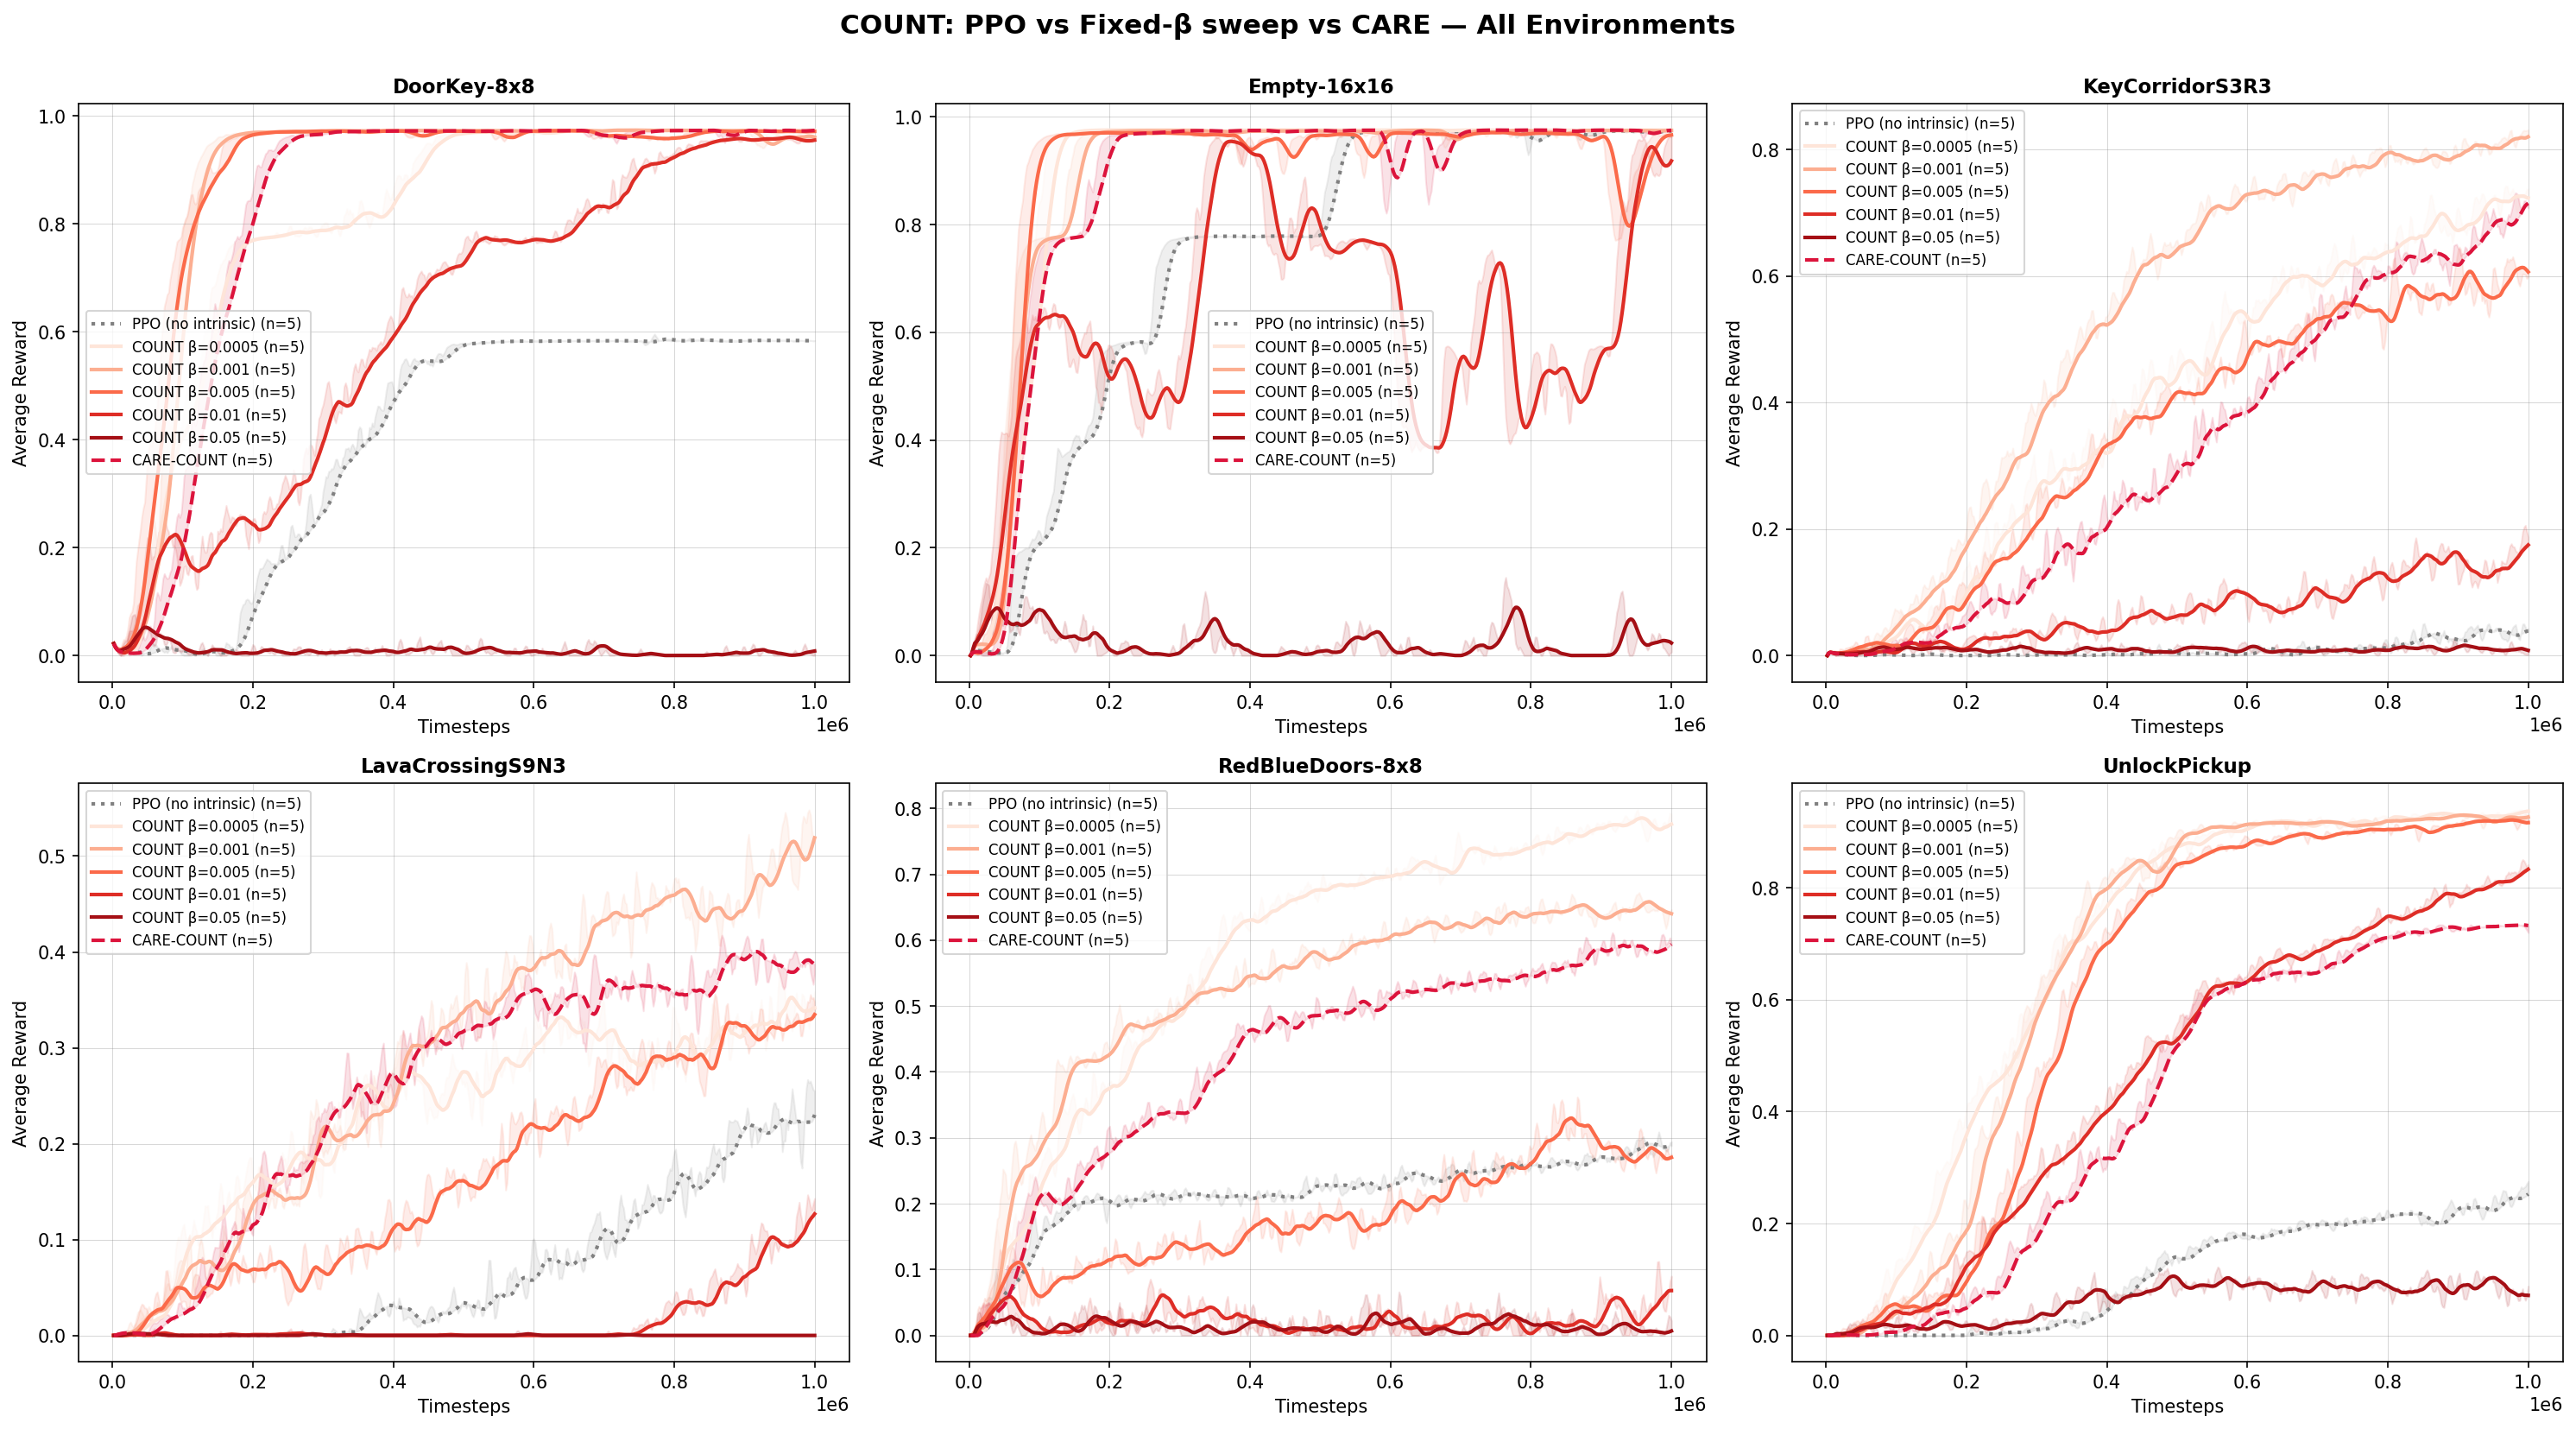
\includegraphics[width=\linewidth]{figures/all_envs_count_beta1e-8_1.png}
\caption[Reward curves for the count-based module (extended bound).]{Reward curves for the count-based module under the extended bounds $[\beta_\text{min},\,\beta_\text{max}] = [10^{-8},\,1]$. Colour conventions follow Figure~\ref{fig:all_envs_count}.}
\label{fig:all_envs_count_ext}
\end{figure}

\begin{figure}[H]
\centering
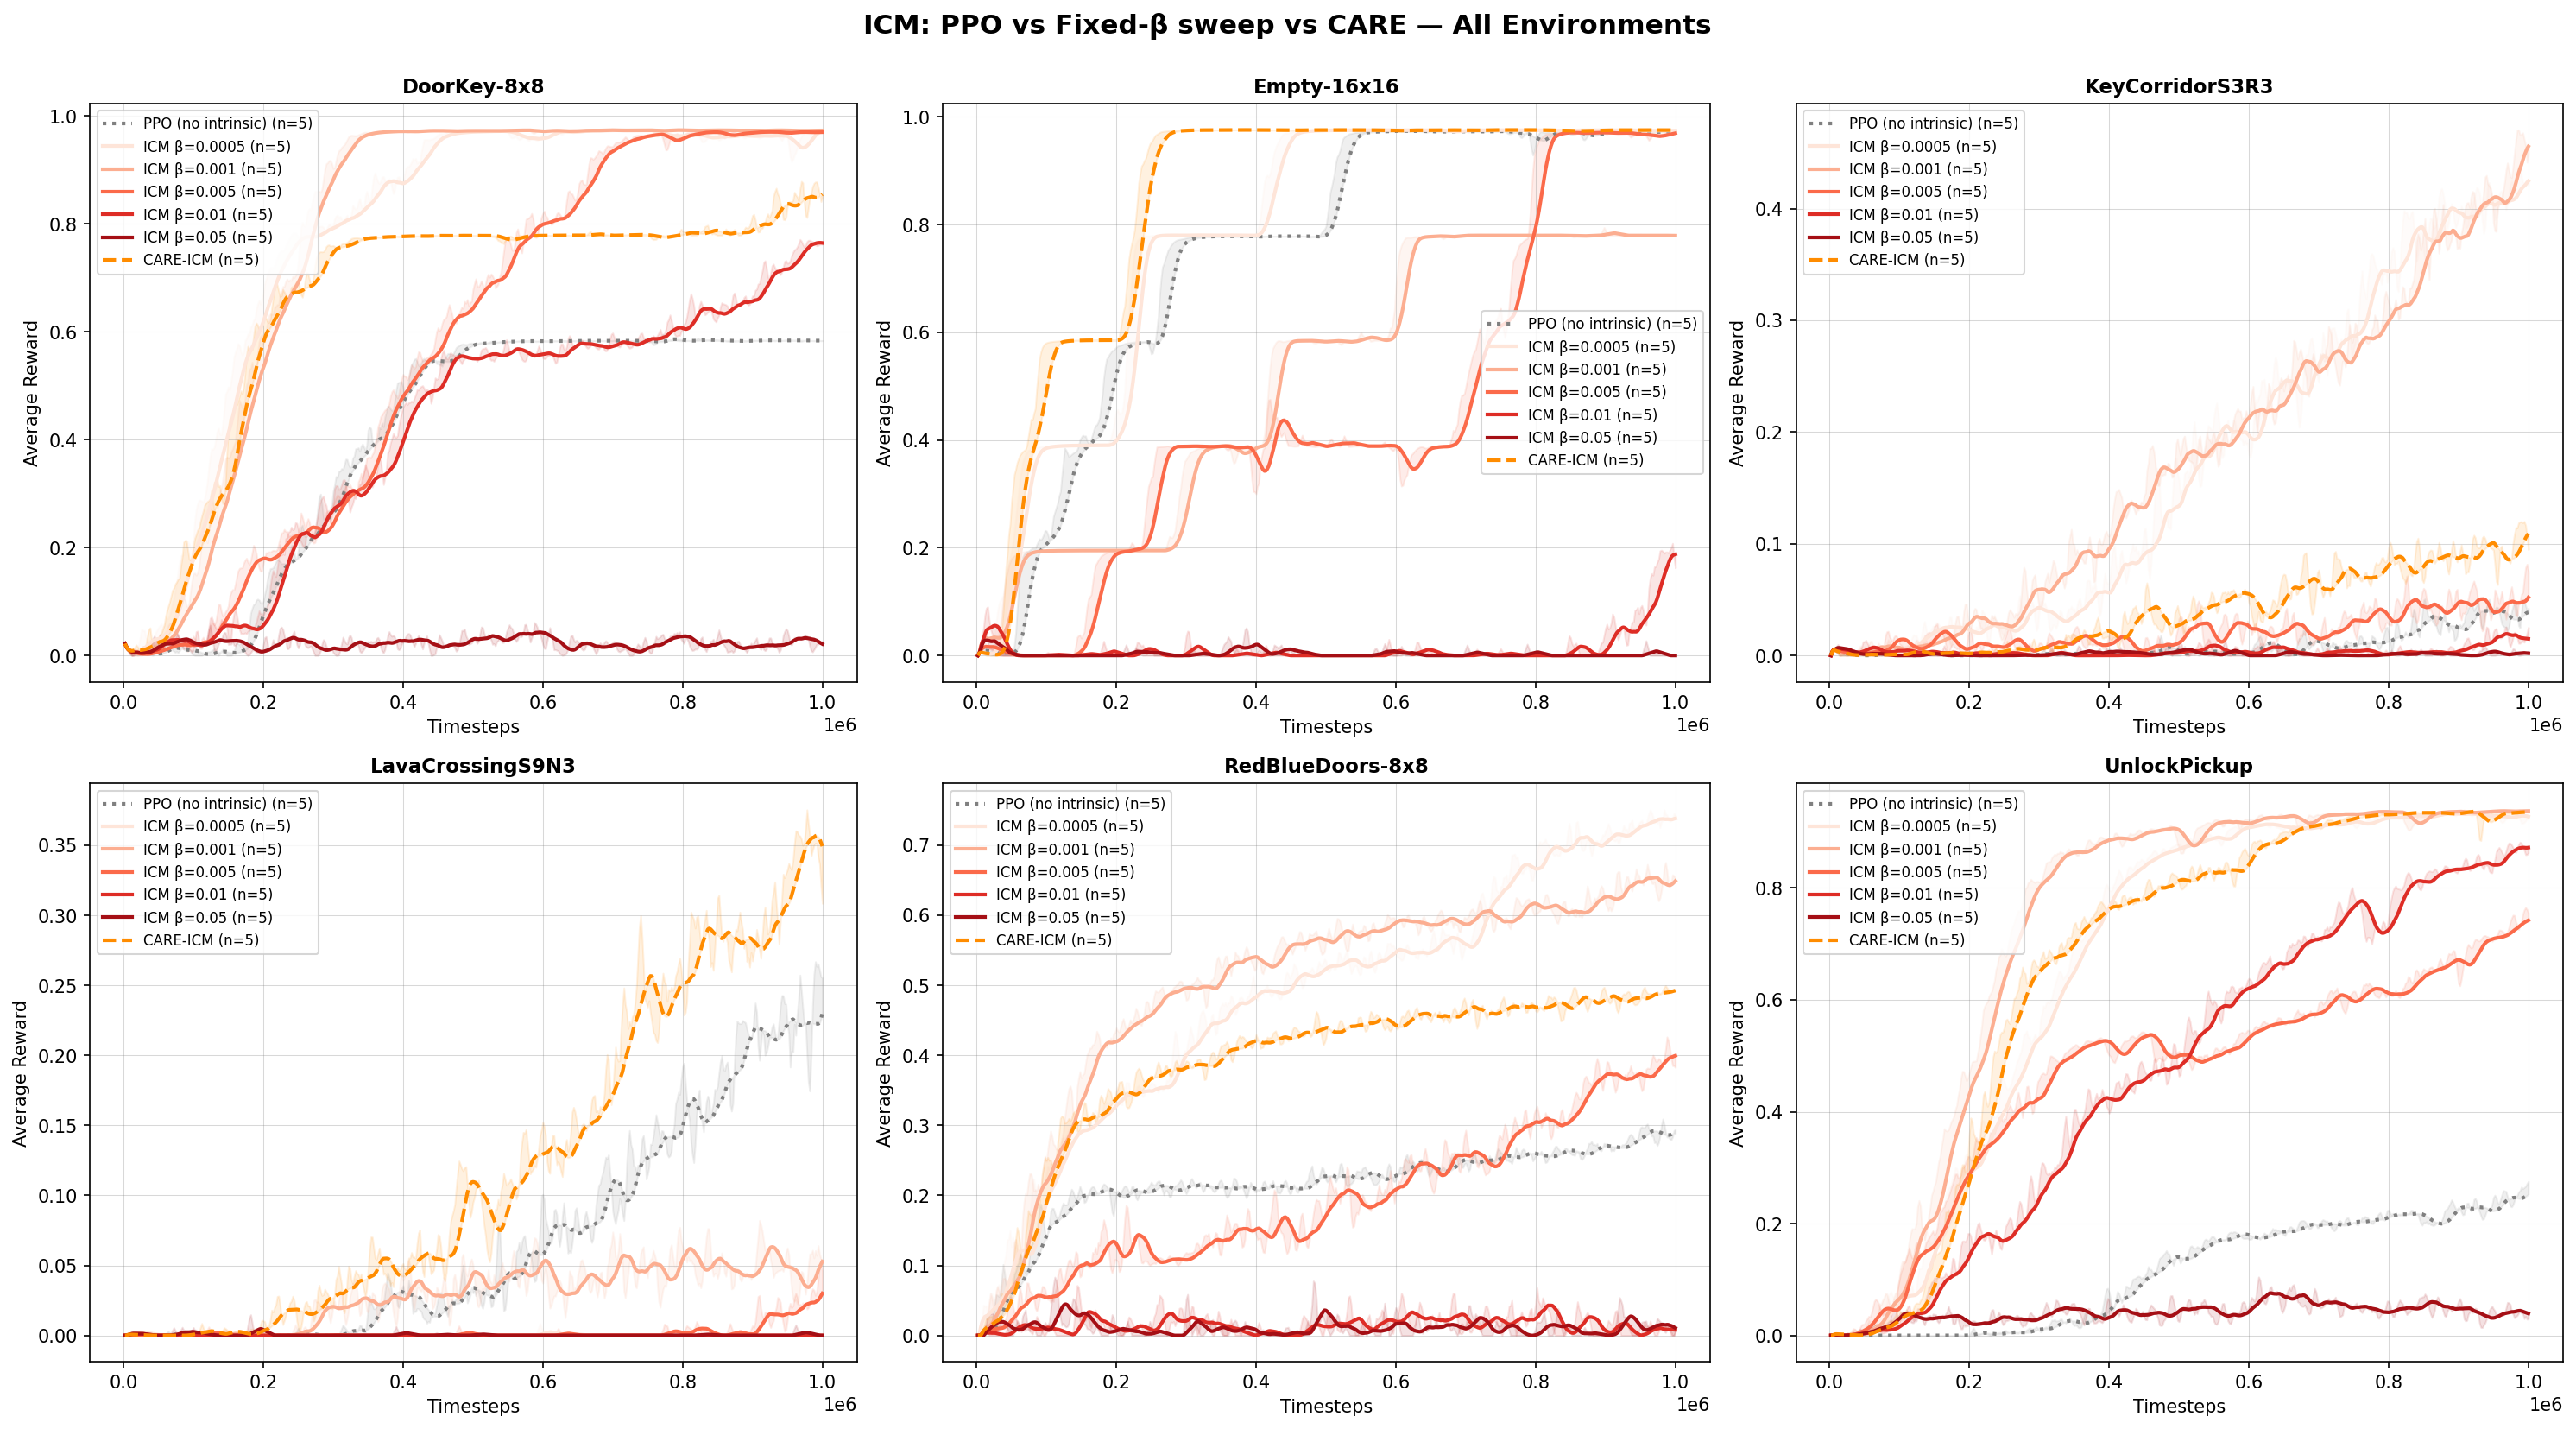
\includegraphics[width=\linewidth]{figures/all_envs_icm_beta1e-8_1.png}
\caption[Reward curves for the ICM module (extended bound).]{Reward curves for the ICM module under the extended bounds. Same colour conventions as Figure~\ref{fig:all_envs_count_ext}.}
\label{fig:all_envs_icm_ext}
\end{figure}

\begin{figure}[H]
\centering
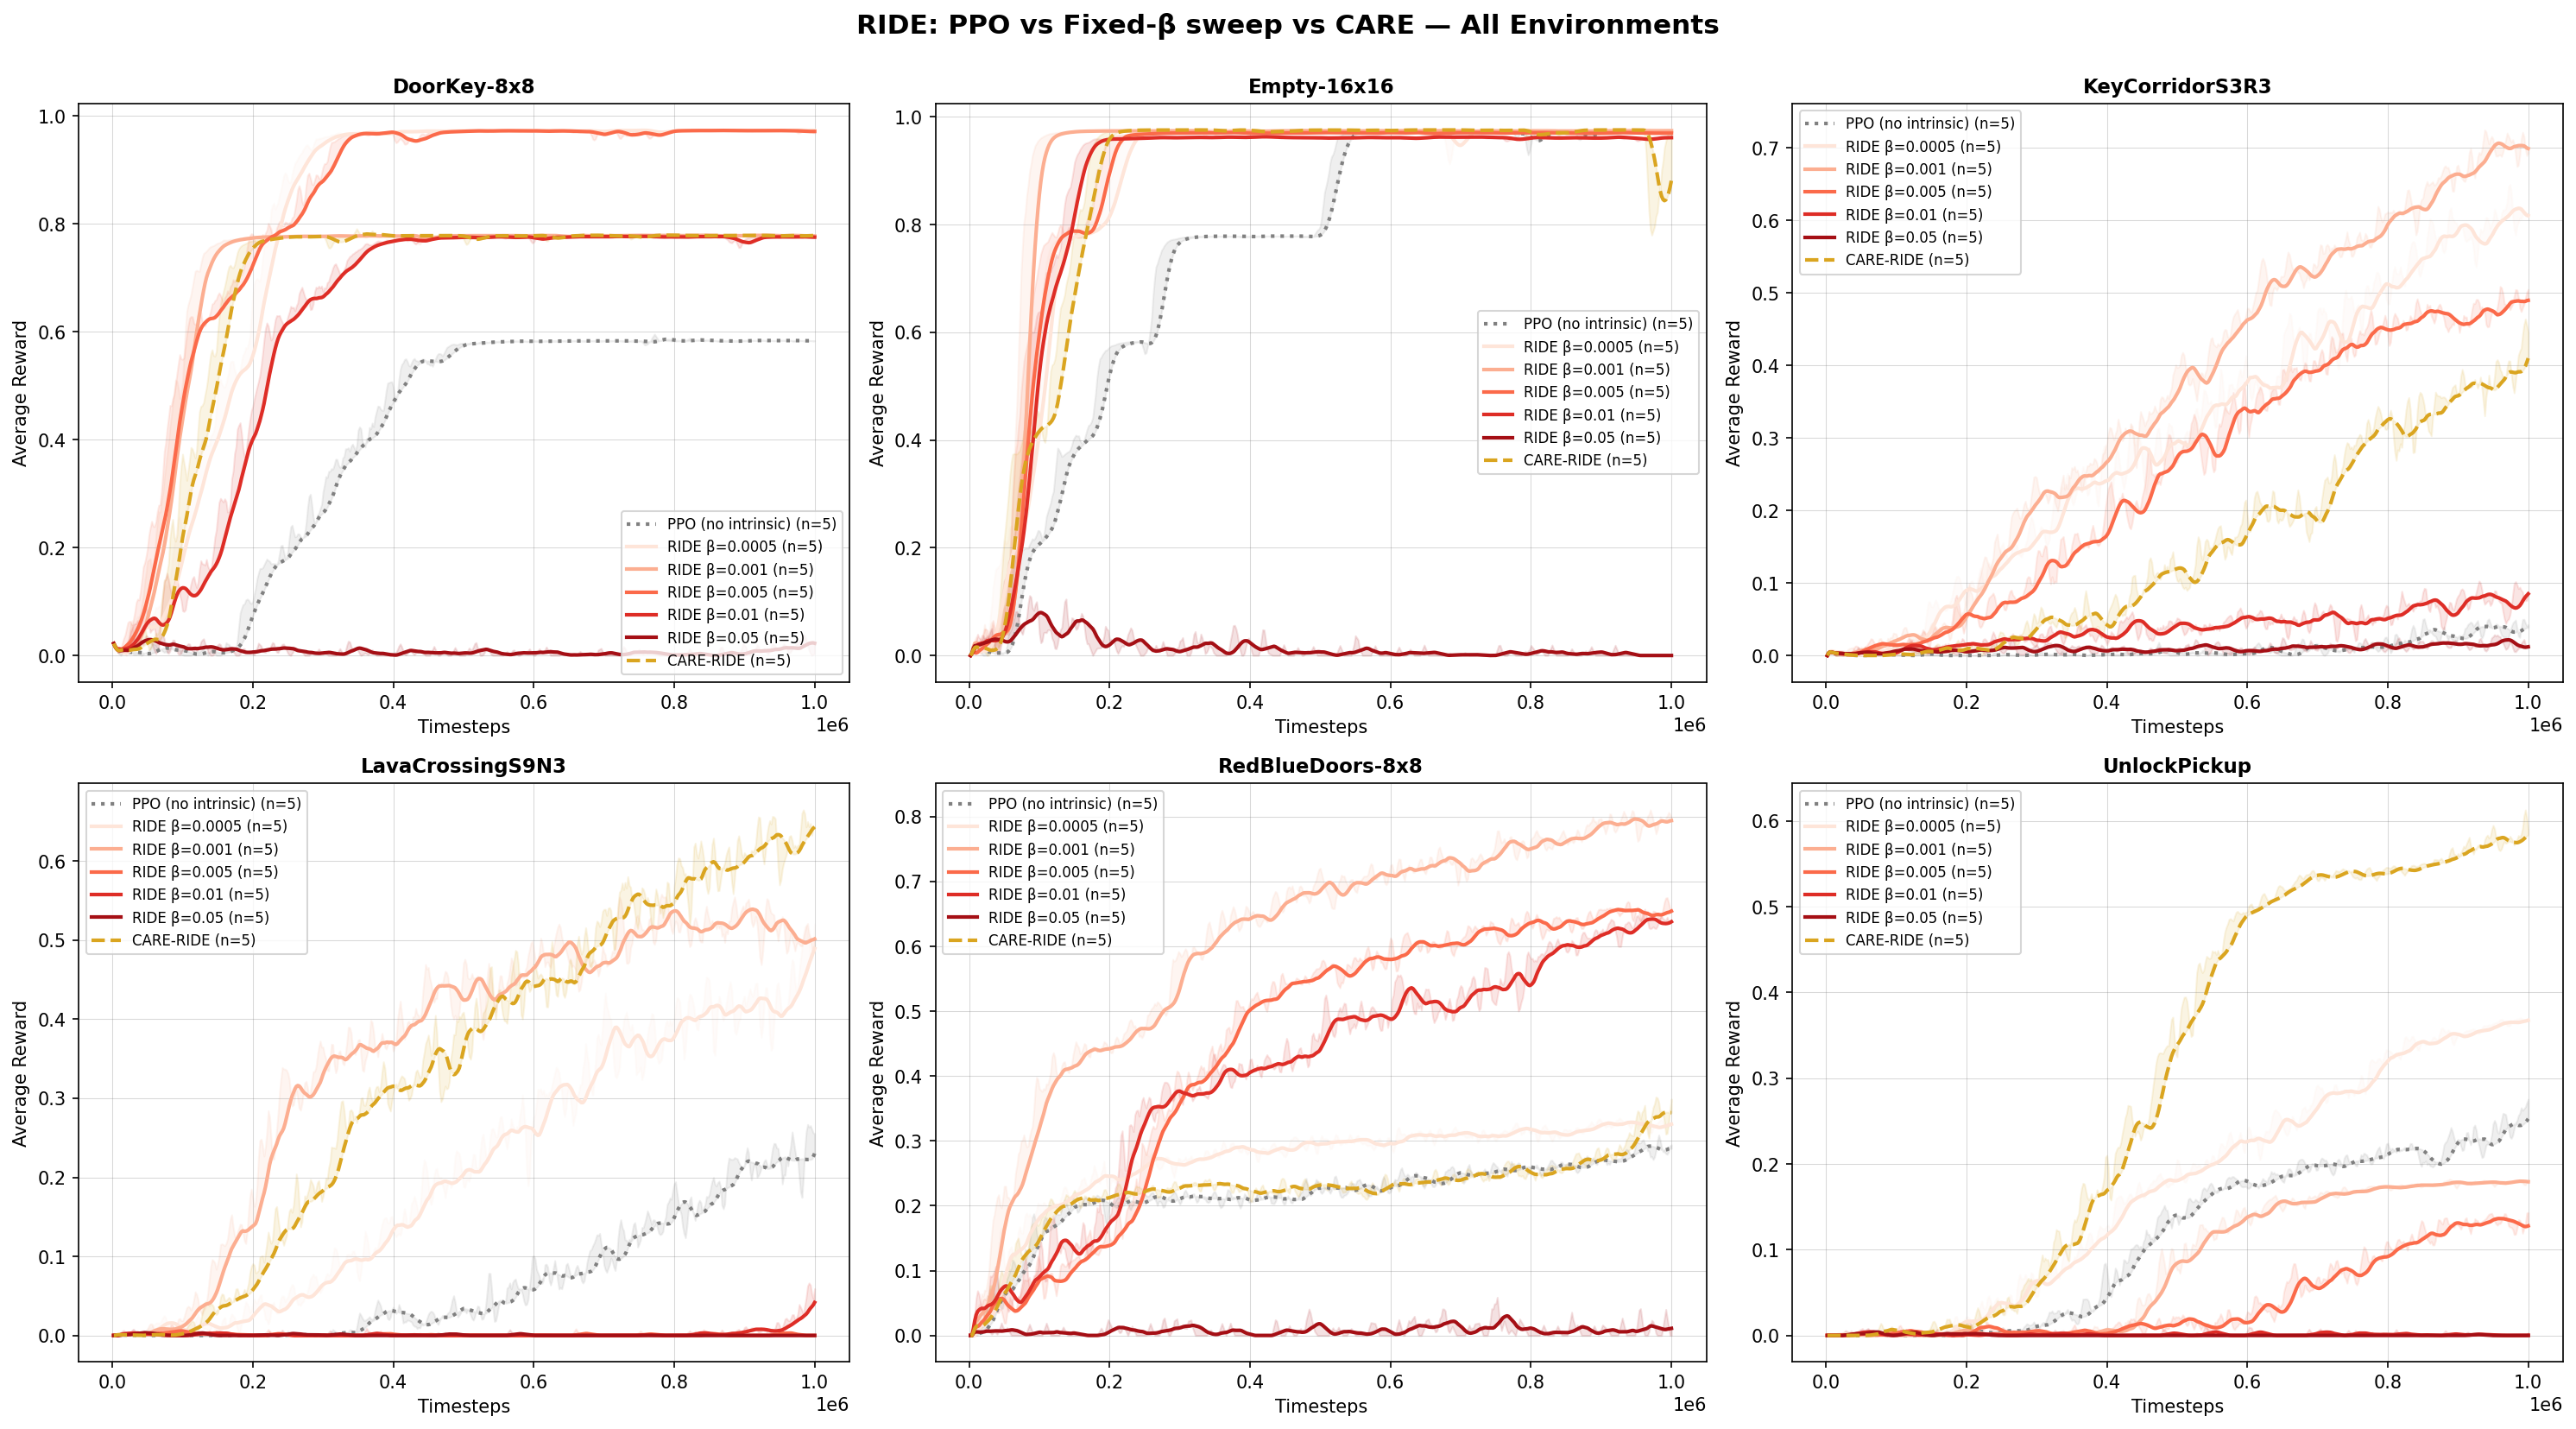
\includegraphics[width=\linewidth]{figures/all_envs_ride_beta1e-8_1.png}
\caption[Reward curves for the RIDE module (extended bound).]{Reward curves for the RIDE module under the extended bounds. Same colour conventions as Figure~\ref{fig:all_envs_count_ext}.}
\label{fig:all_envs_ride_ext}
\end{figure}

\section{Aggregate Performance}
\label{sec:ext_beta_aggregate}

\begin{figure}[H]
\centering
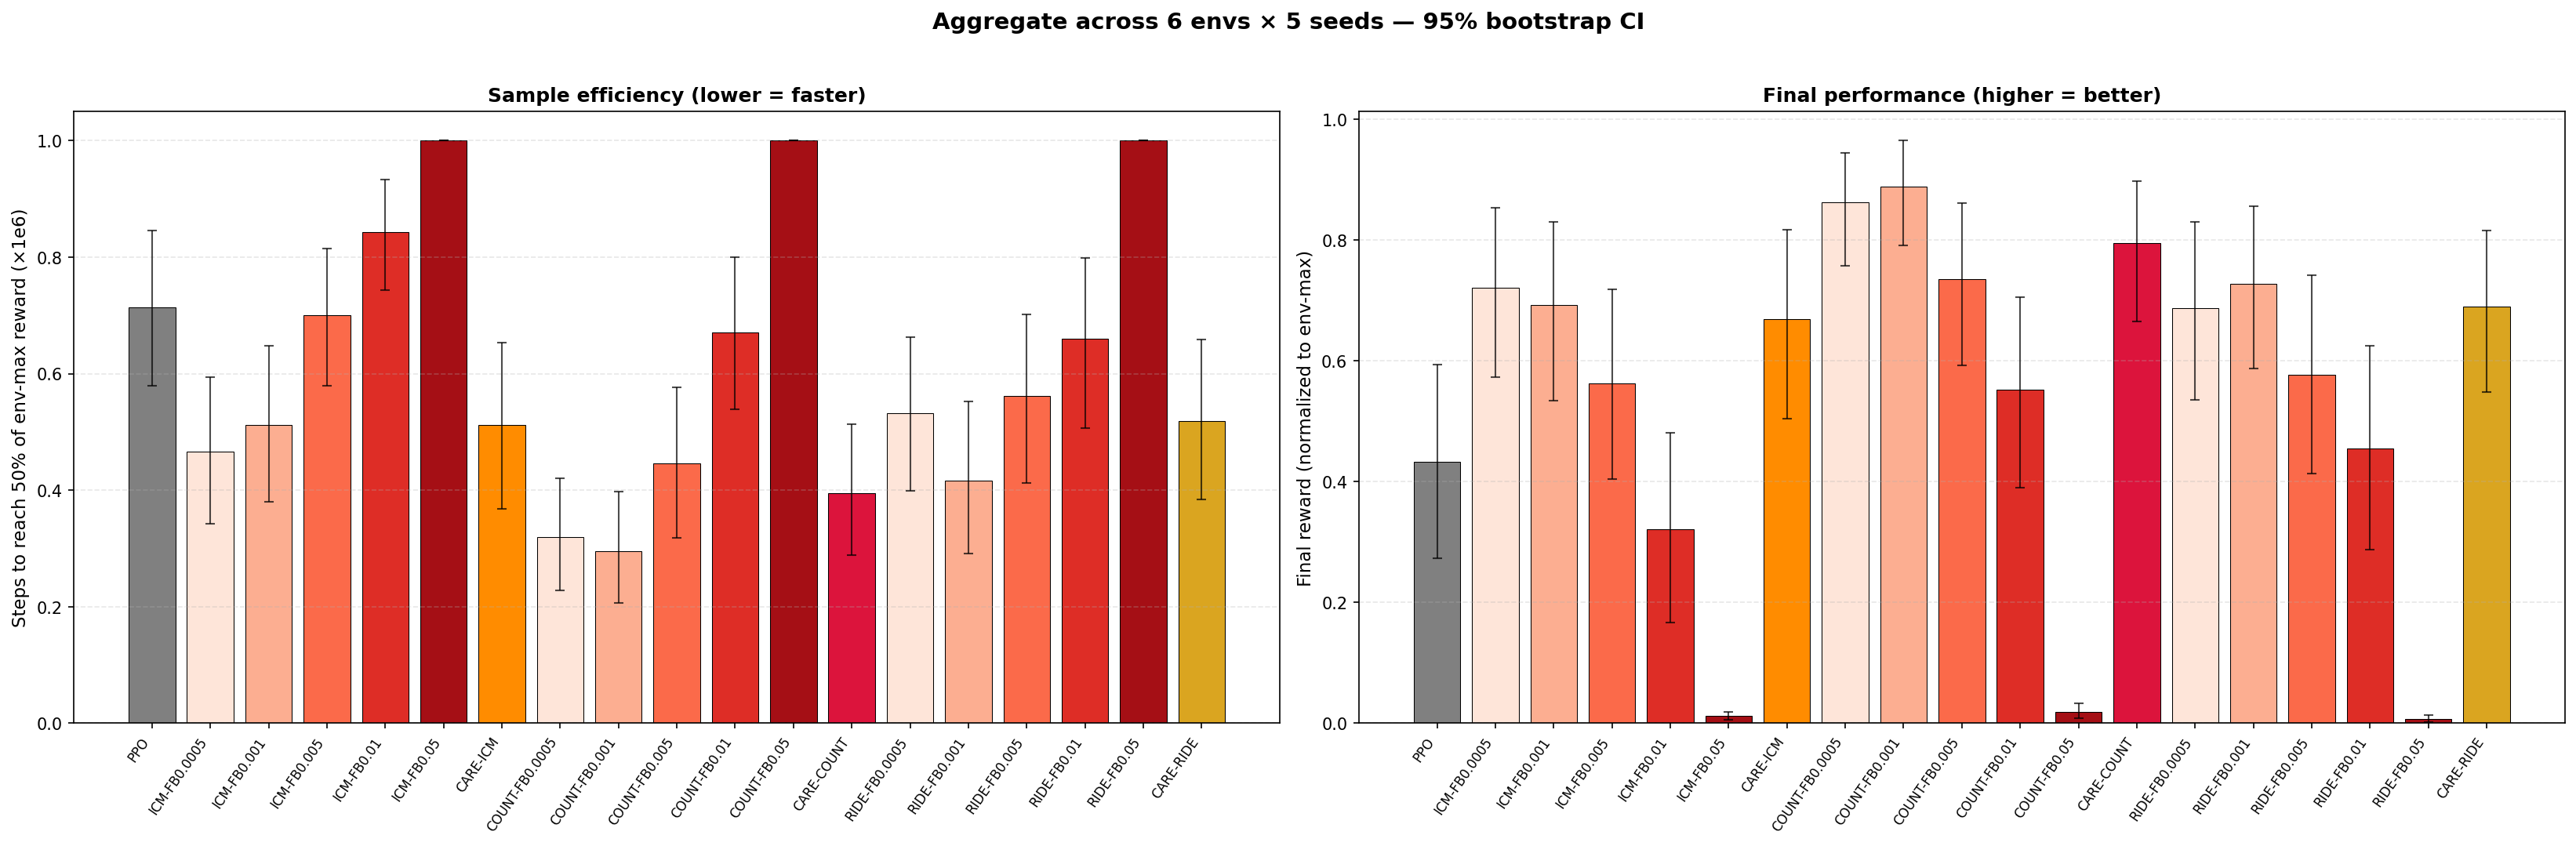
\includegraphics[width=\linewidth]{figures/aggregate_summary_beta1e-8_1.png}
\caption[Aggregate performance summary (extended bound).]{Aggregate performance summary under the extended bounds. Conventions follow Figure~\ref{fig:aggregate_summary}.}
\label{fig:aggregate_summary_ext}
\end{figure}

\begin{figure}[H]
\centering
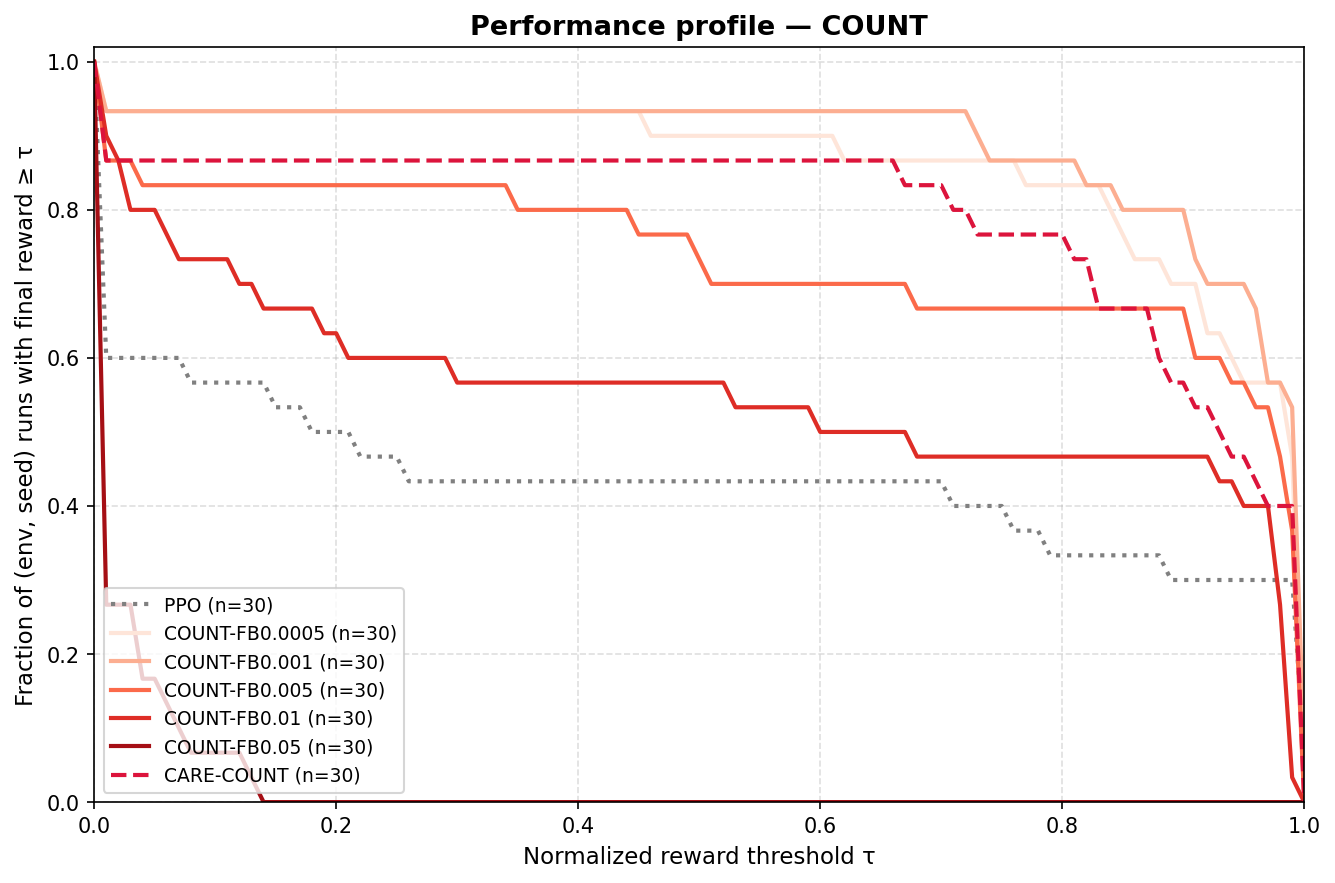
\includegraphics[width=\linewidth]{figures/profile_count_beta1e-8_1.png}
\caption[Performance profile, count-based module (extended bound).]{Performance profile for the count-based module under the extended bounds. Same conventions as Figure~\ref{fig:profile_count}.}
\label{fig:profile_count_ext}
\end{figure}

\begin{figure}[H]
\centering
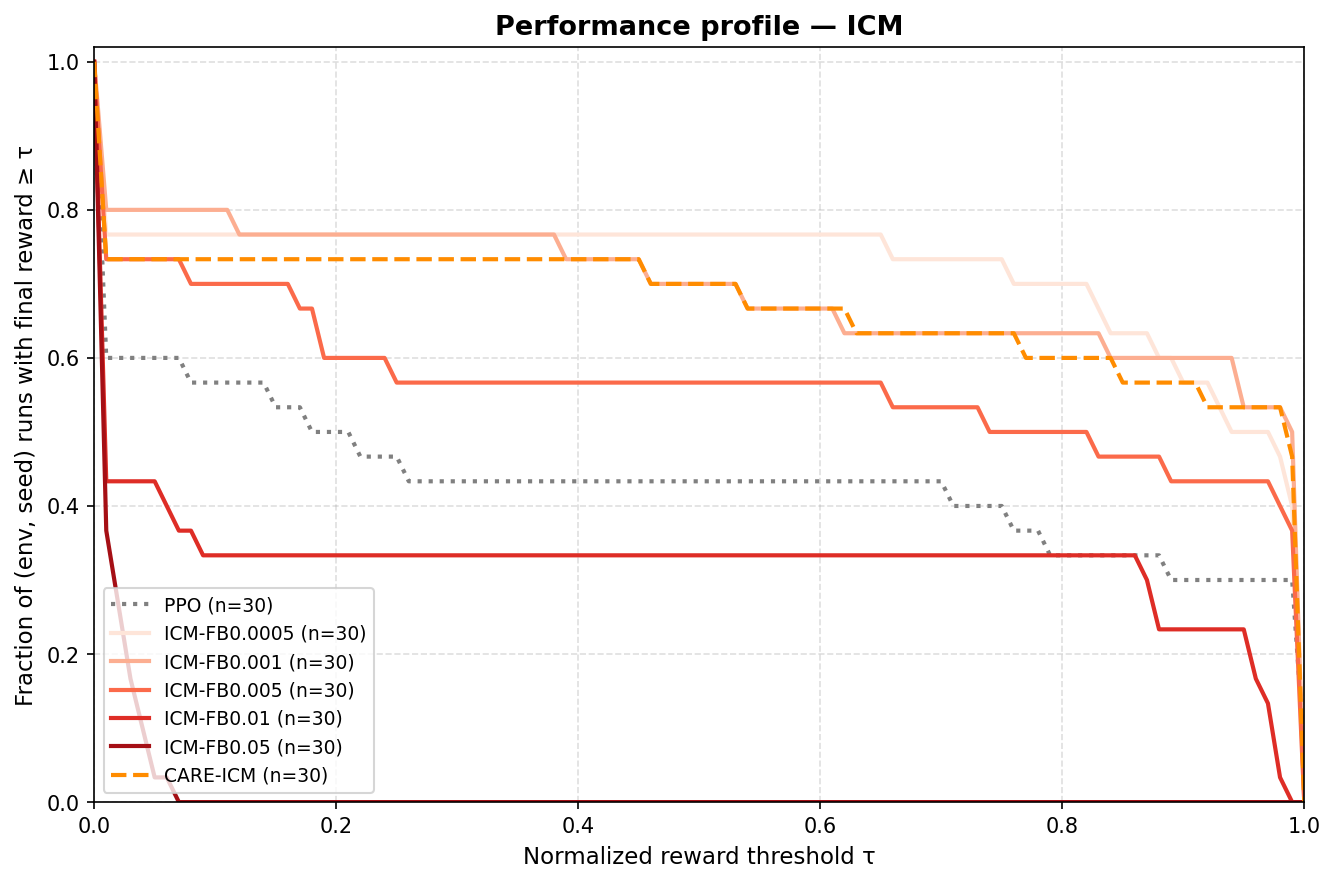
\includegraphics[width=\linewidth]{figures/profile_icm_beta1e-8_1.png}
\caption[Performance profile, ICM module (extended bound).]{Performance profile for the ICM module under the extended bounds. Same conventions as Figure~\ref{fig:profile_count_ext}.}
\label{fig:profile_icm_ext}
\end{figure}

\begin{figure}[H]
\centering
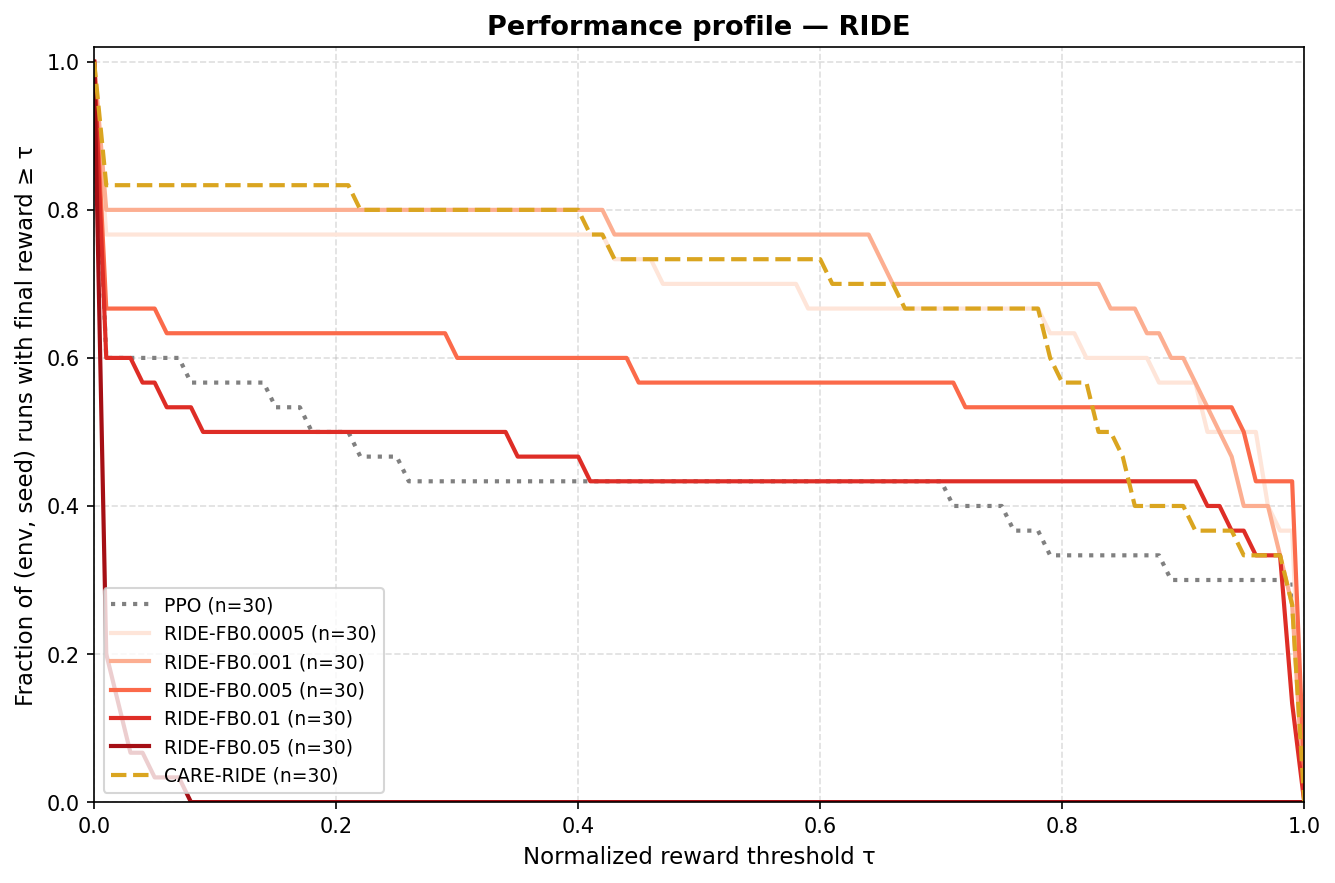
\includegraphics[width=\linewidth]{figures/profile_ride_beta1e-8_1.png}
\caption[Performance profile, RIDE module (extended bound).]{Performance profile for the RIDE module under the extended bounds. Same conventions as Figure~\ref{fig:profile_count_ext}.}
\label{fig:profile_ride_ext}
\end{figure}

\section{CARE Dynamics and $\beta_\psi$ Distribution}
\label{sec:ext_beta_dynamics}

\begin{figure}[H]
\centering
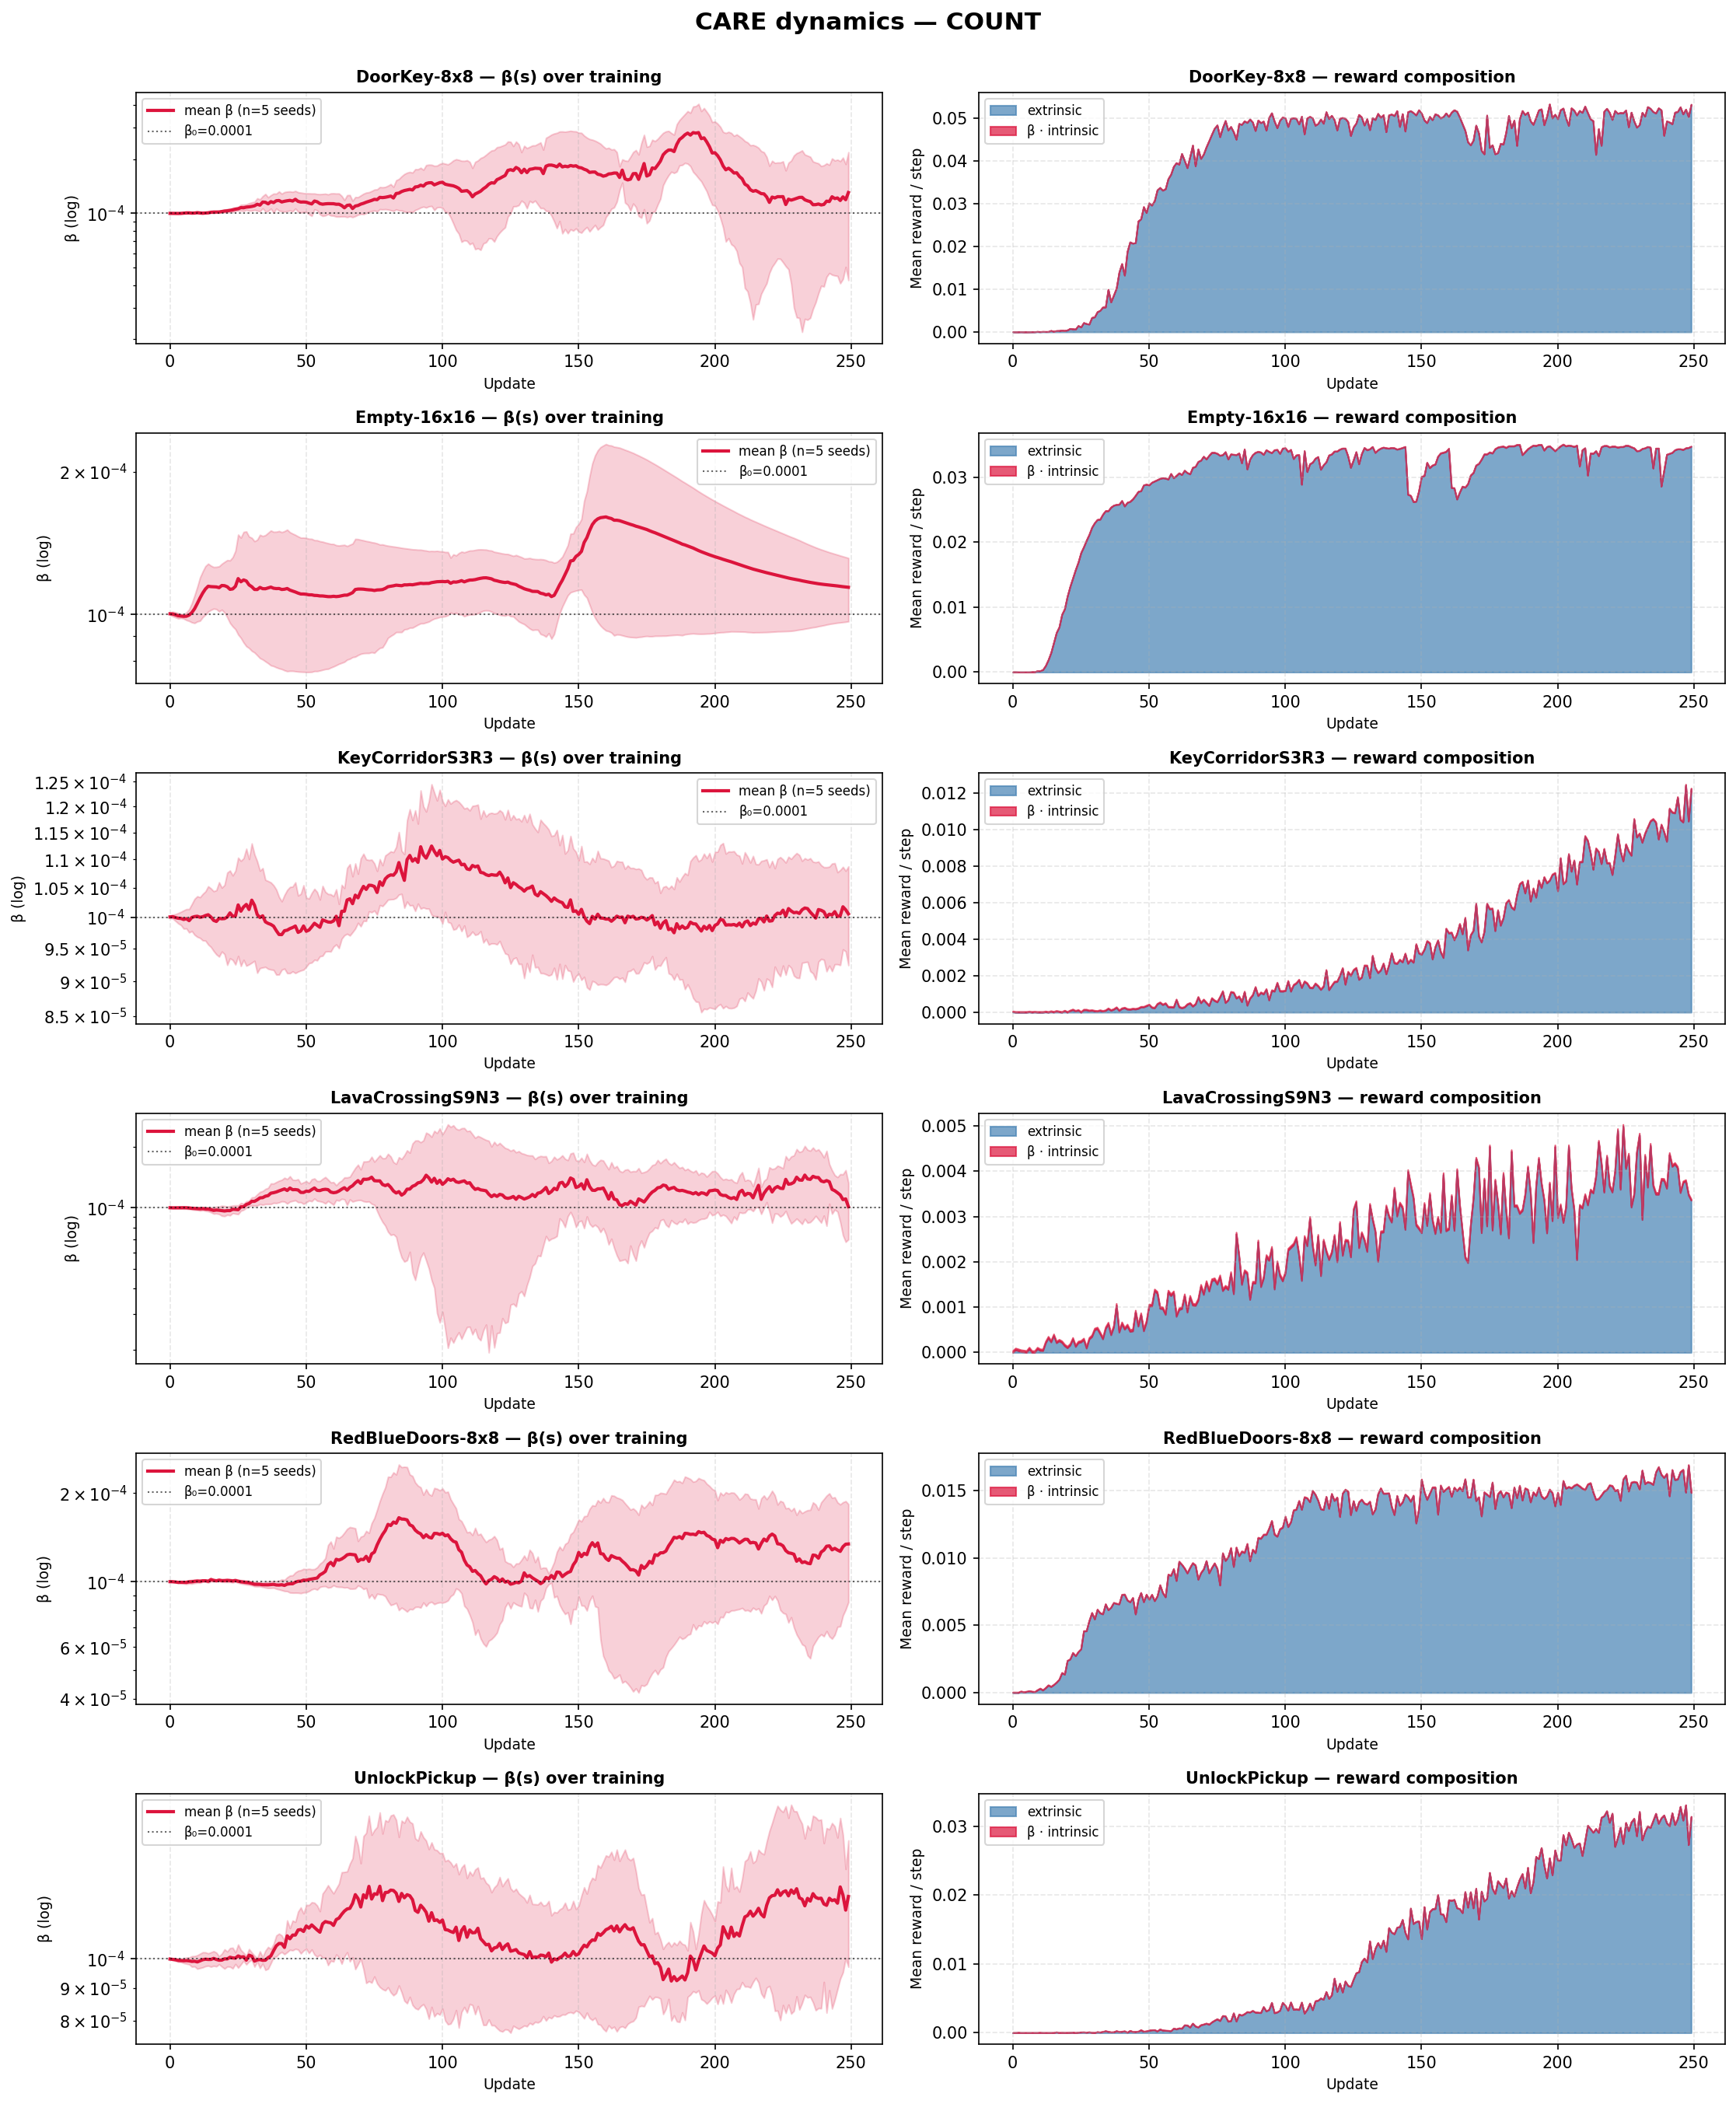
\includegraphics[width=\linewidth]{figures/care_dynamics_count_beta1e-8_1.png}
\caption[CARE-COUNT dynamics (extended bound).]{CARE-COUNT dynamics under the extended bounds. Same panel layout as Figure~\ref{fig:care_dynamics_count}; the left-panel $\beta_\psi$ axis now spans the wider interval $[10^{-8},\,1]$.}
\label{fig:care_dynamics_count_ext}
\end{figure}

\begin{figure}[H]
\centering
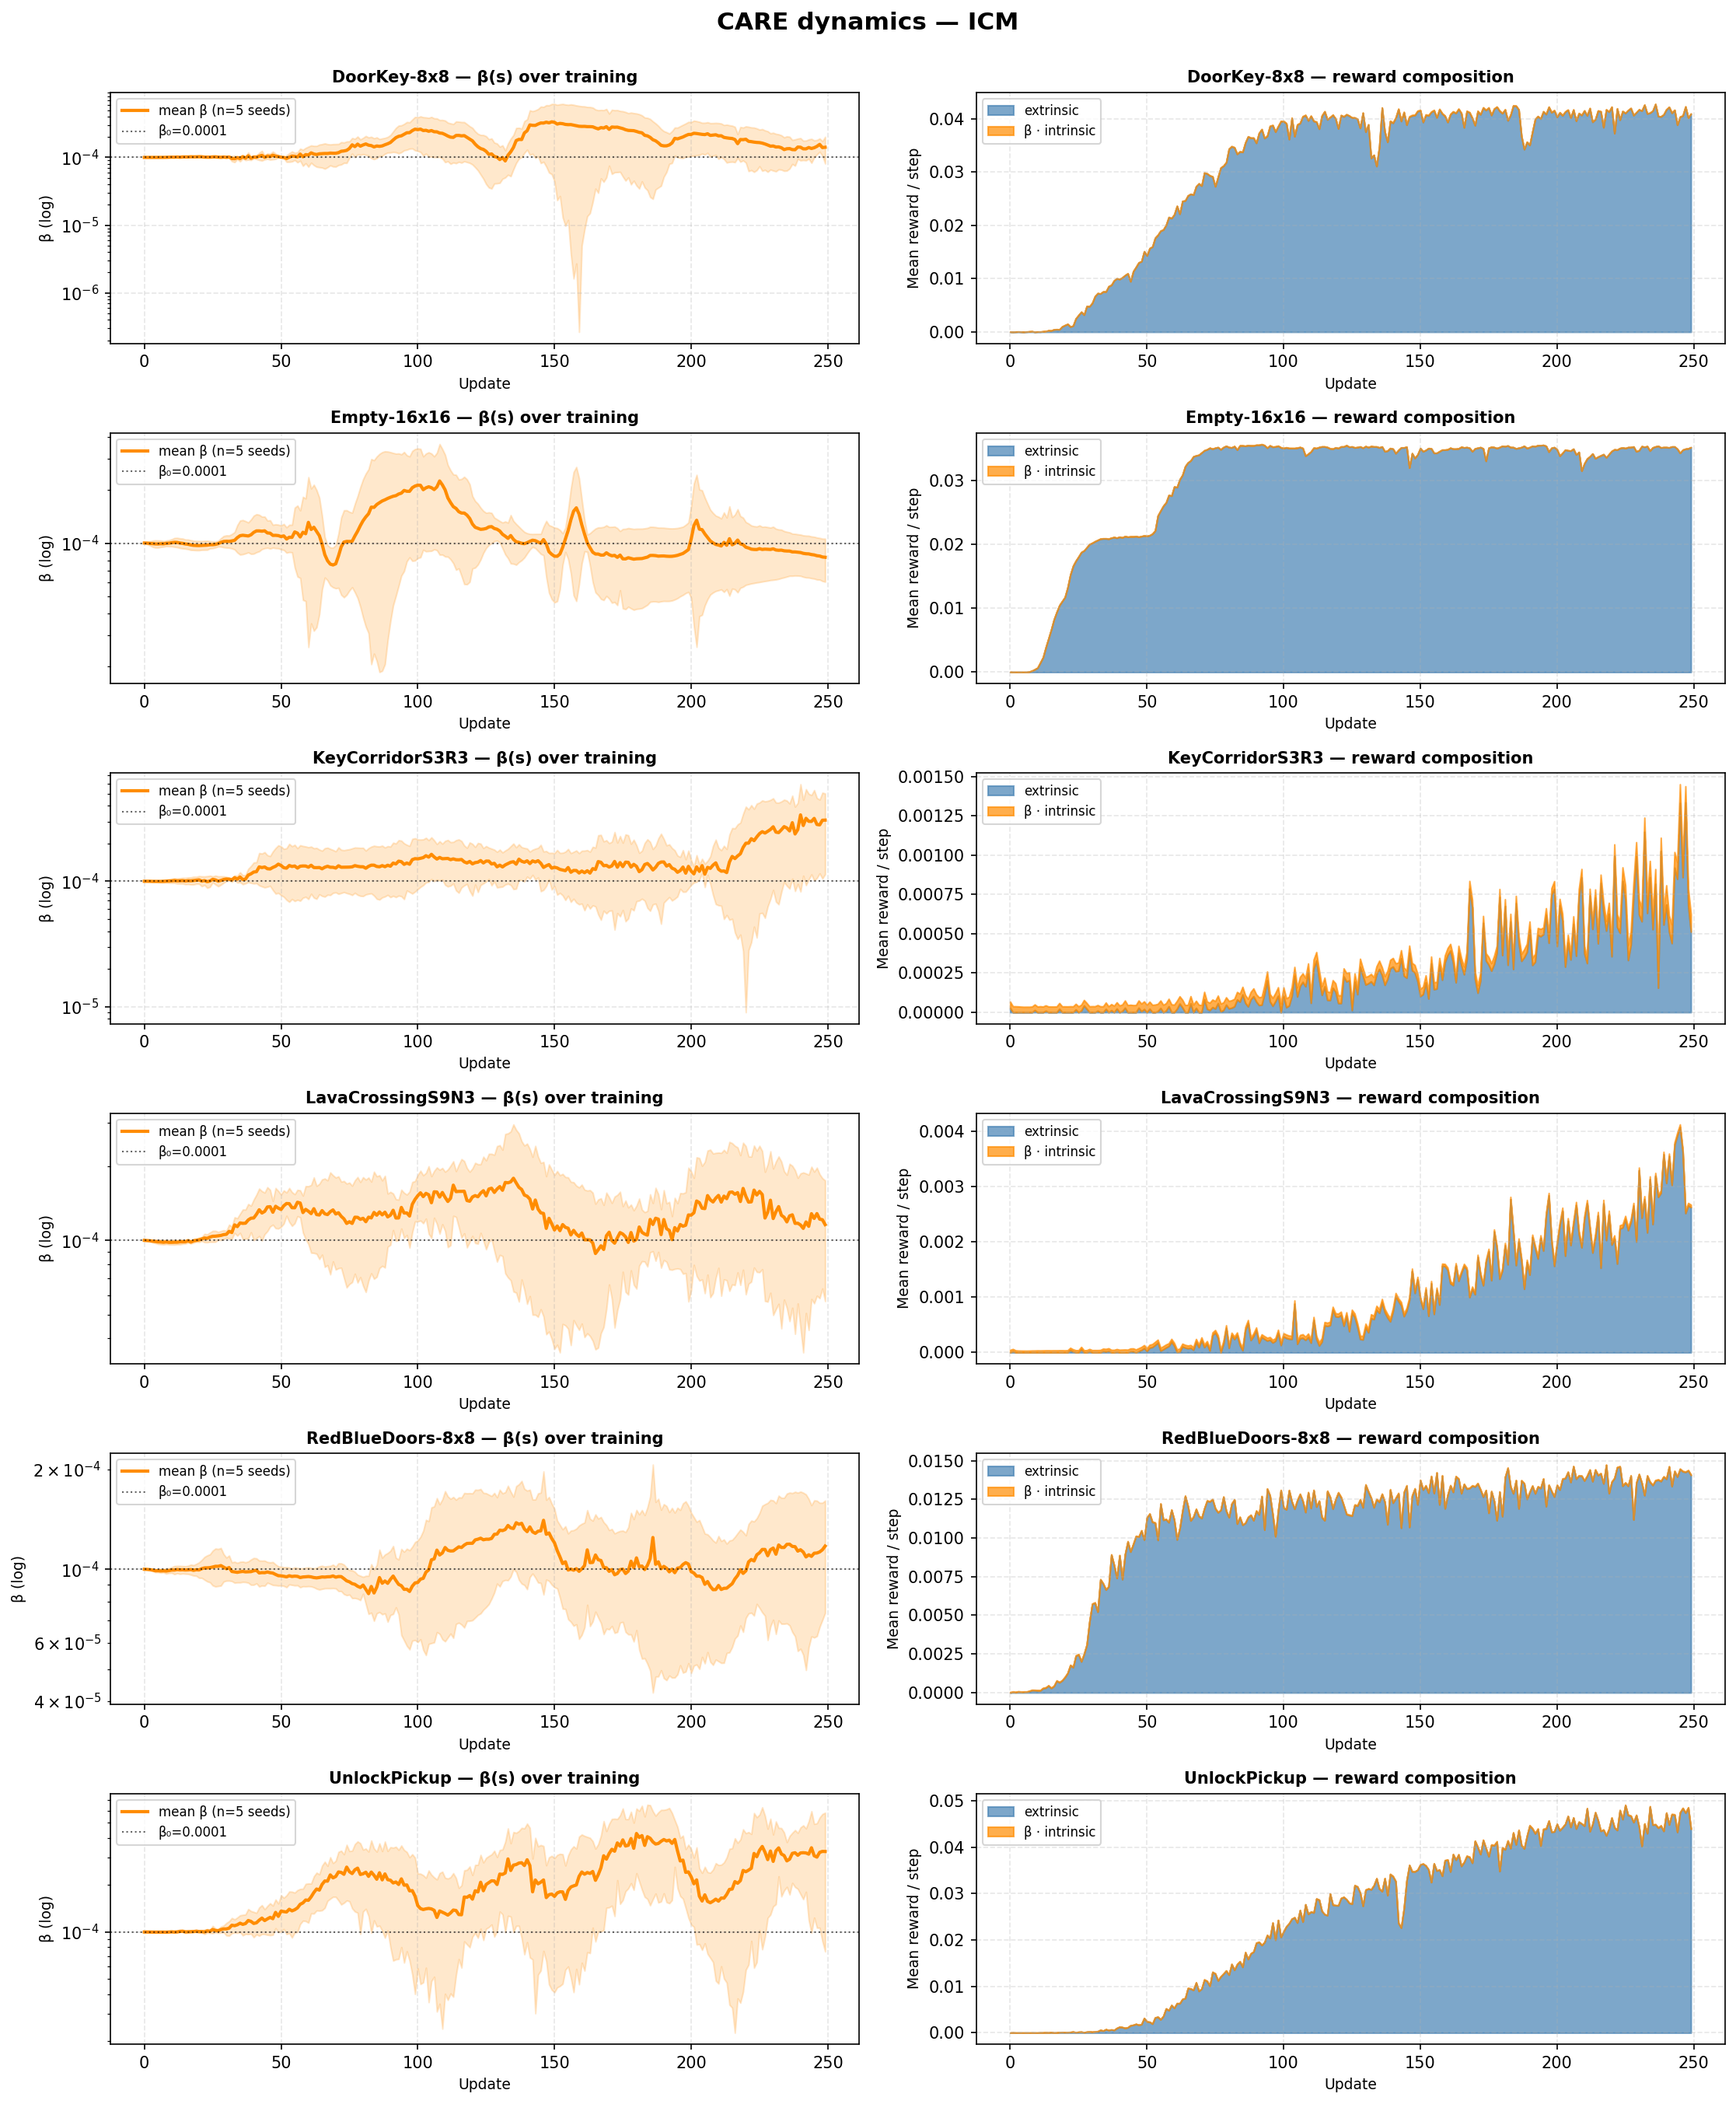
\includegraphics[width=\linewidth]{figures/care_dynamics_icm_beta1e-8_1.png}
\caption[CARE-ICM dynamics (extended bound).]{CARE-ICM dynamics under the extended bounds. Same conventions as Figure~\ref{fig:care_dynamics_count_ext}.}
\label{fig:care_dynamics_icm_ext}
\end{figure}

\begin{figure}[H]
\centering
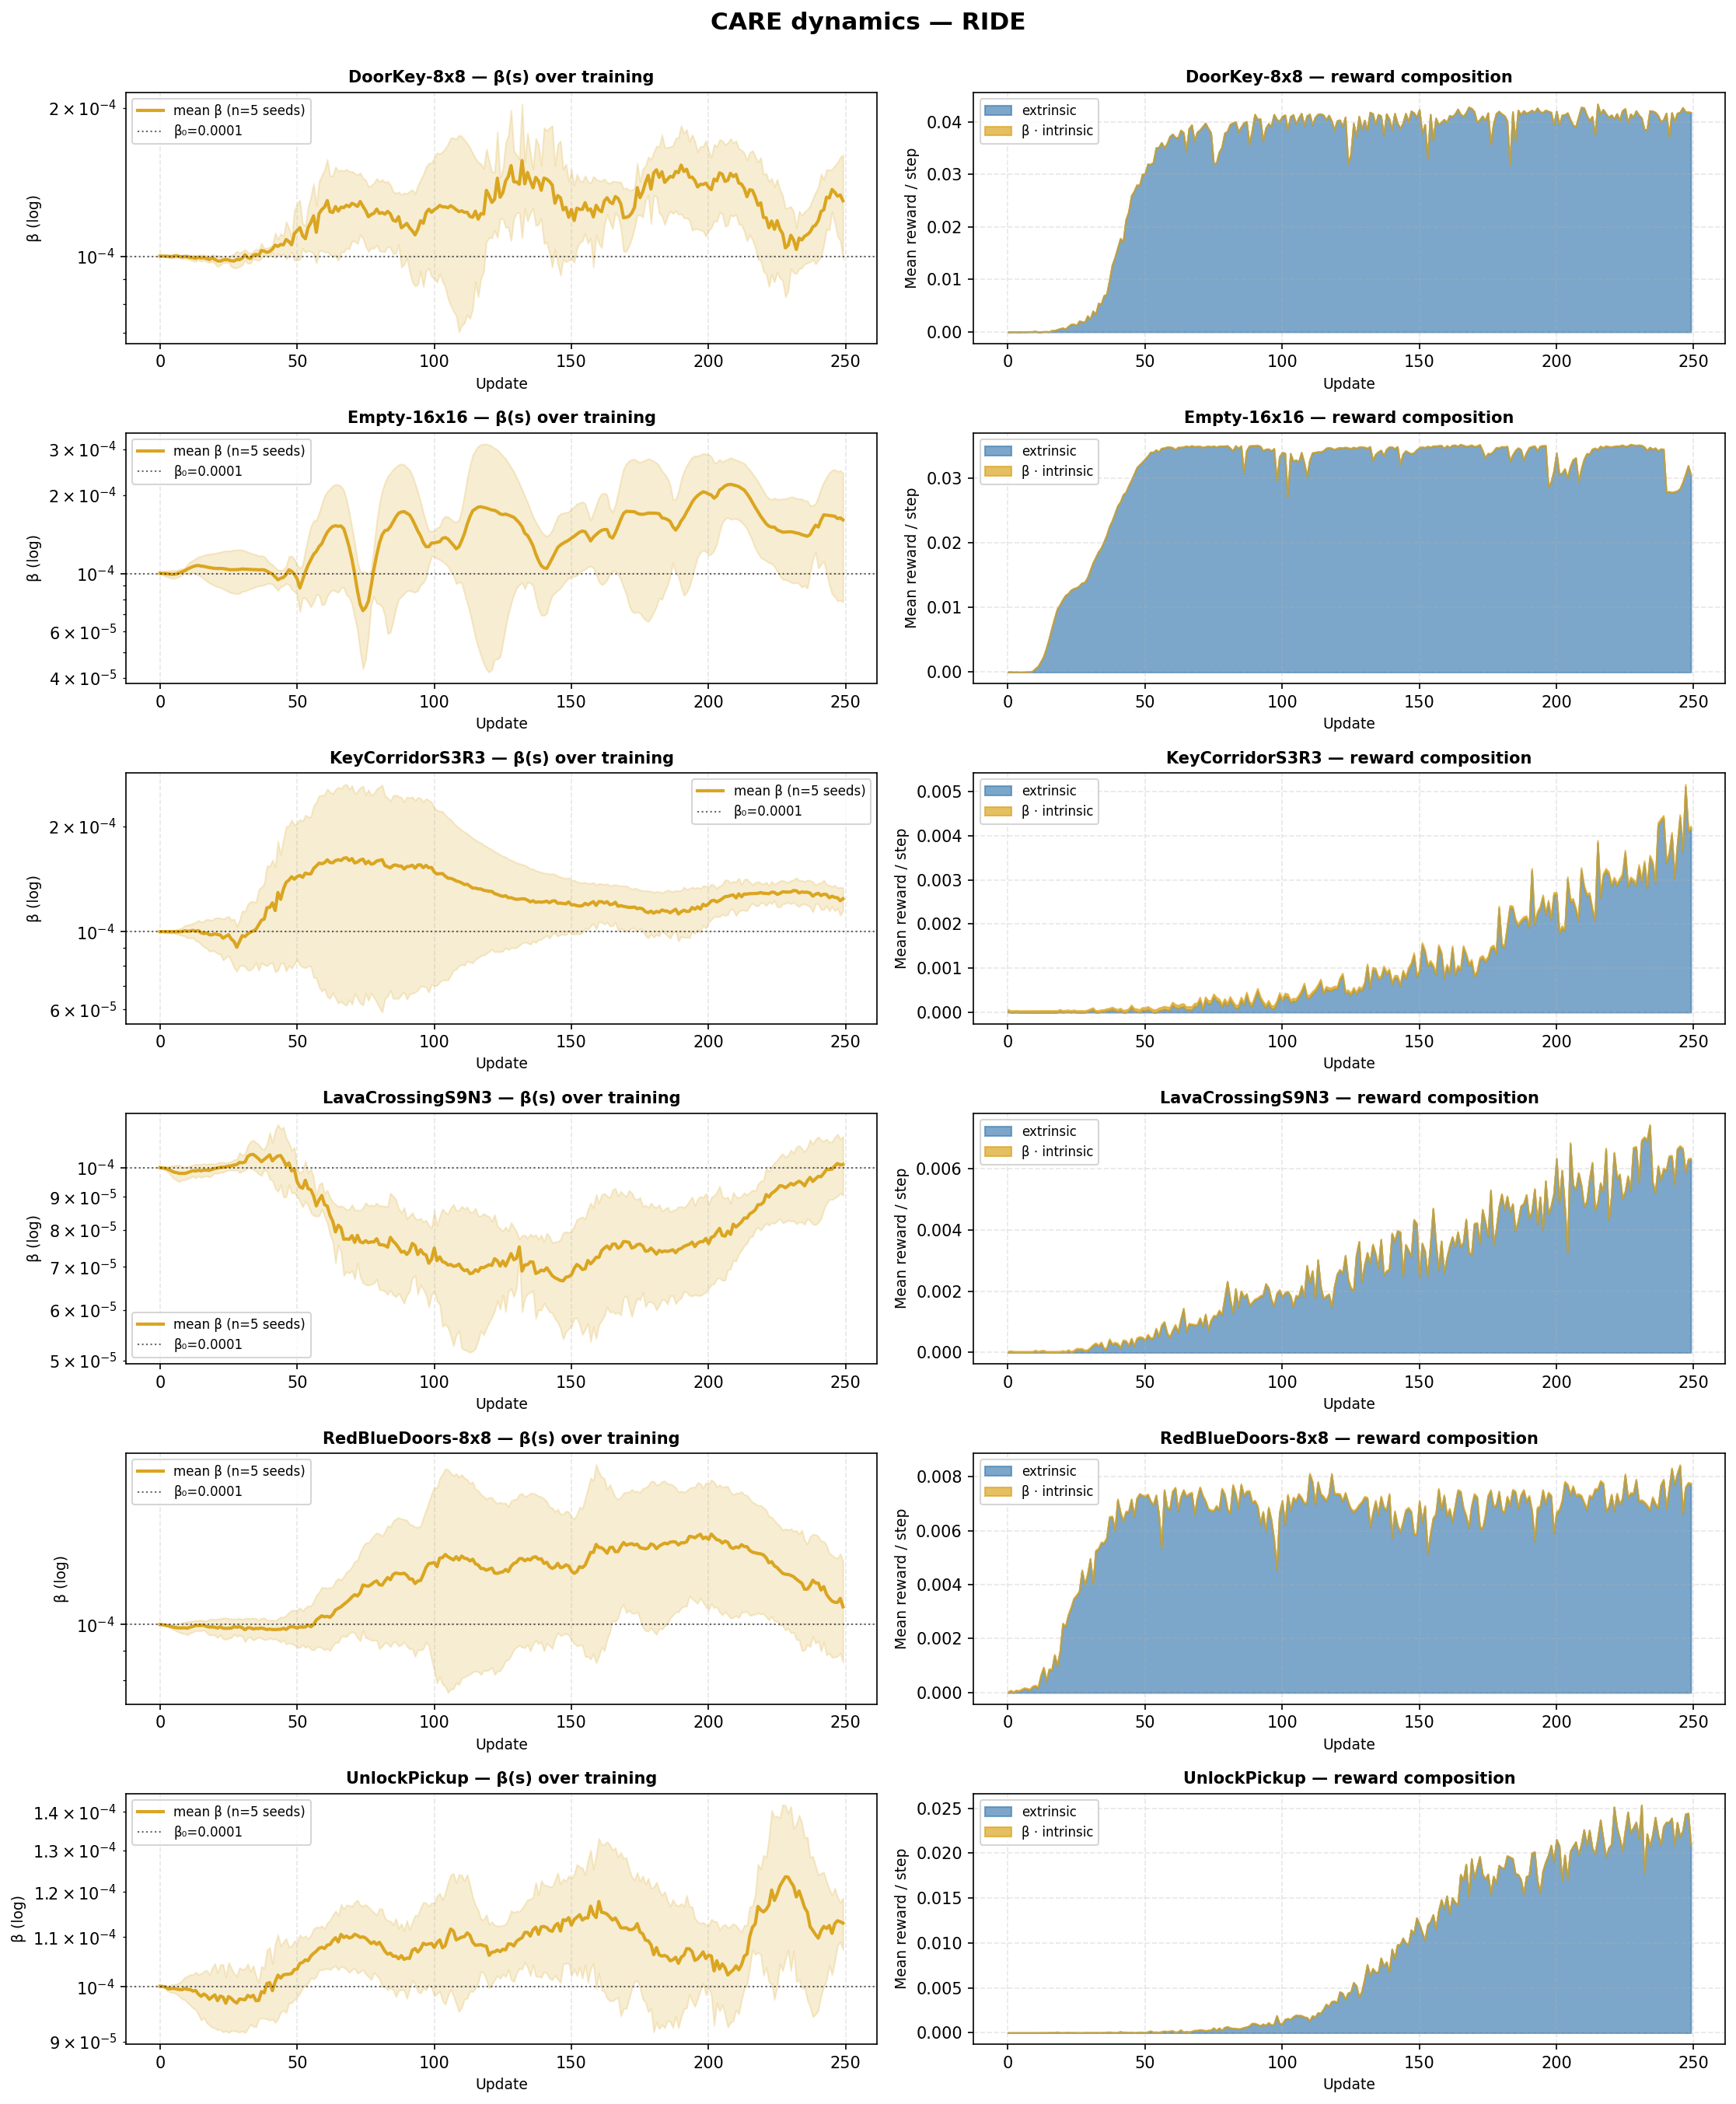
\includegraphics[width=\linewidth]{figures/care_dynamics_ride_beta1e-8_1.png}
\caption[CARE-RIDE dynamics (extended bound).]{CARE-RIDE dynamics under the extended bounds. Same conventions as Figure~\ref{fig:care_dynamics_count_ext}.}
\label{fig:care_dynamics_ride_ext}
\end{figure}

\begin{figure}[H]
\centering
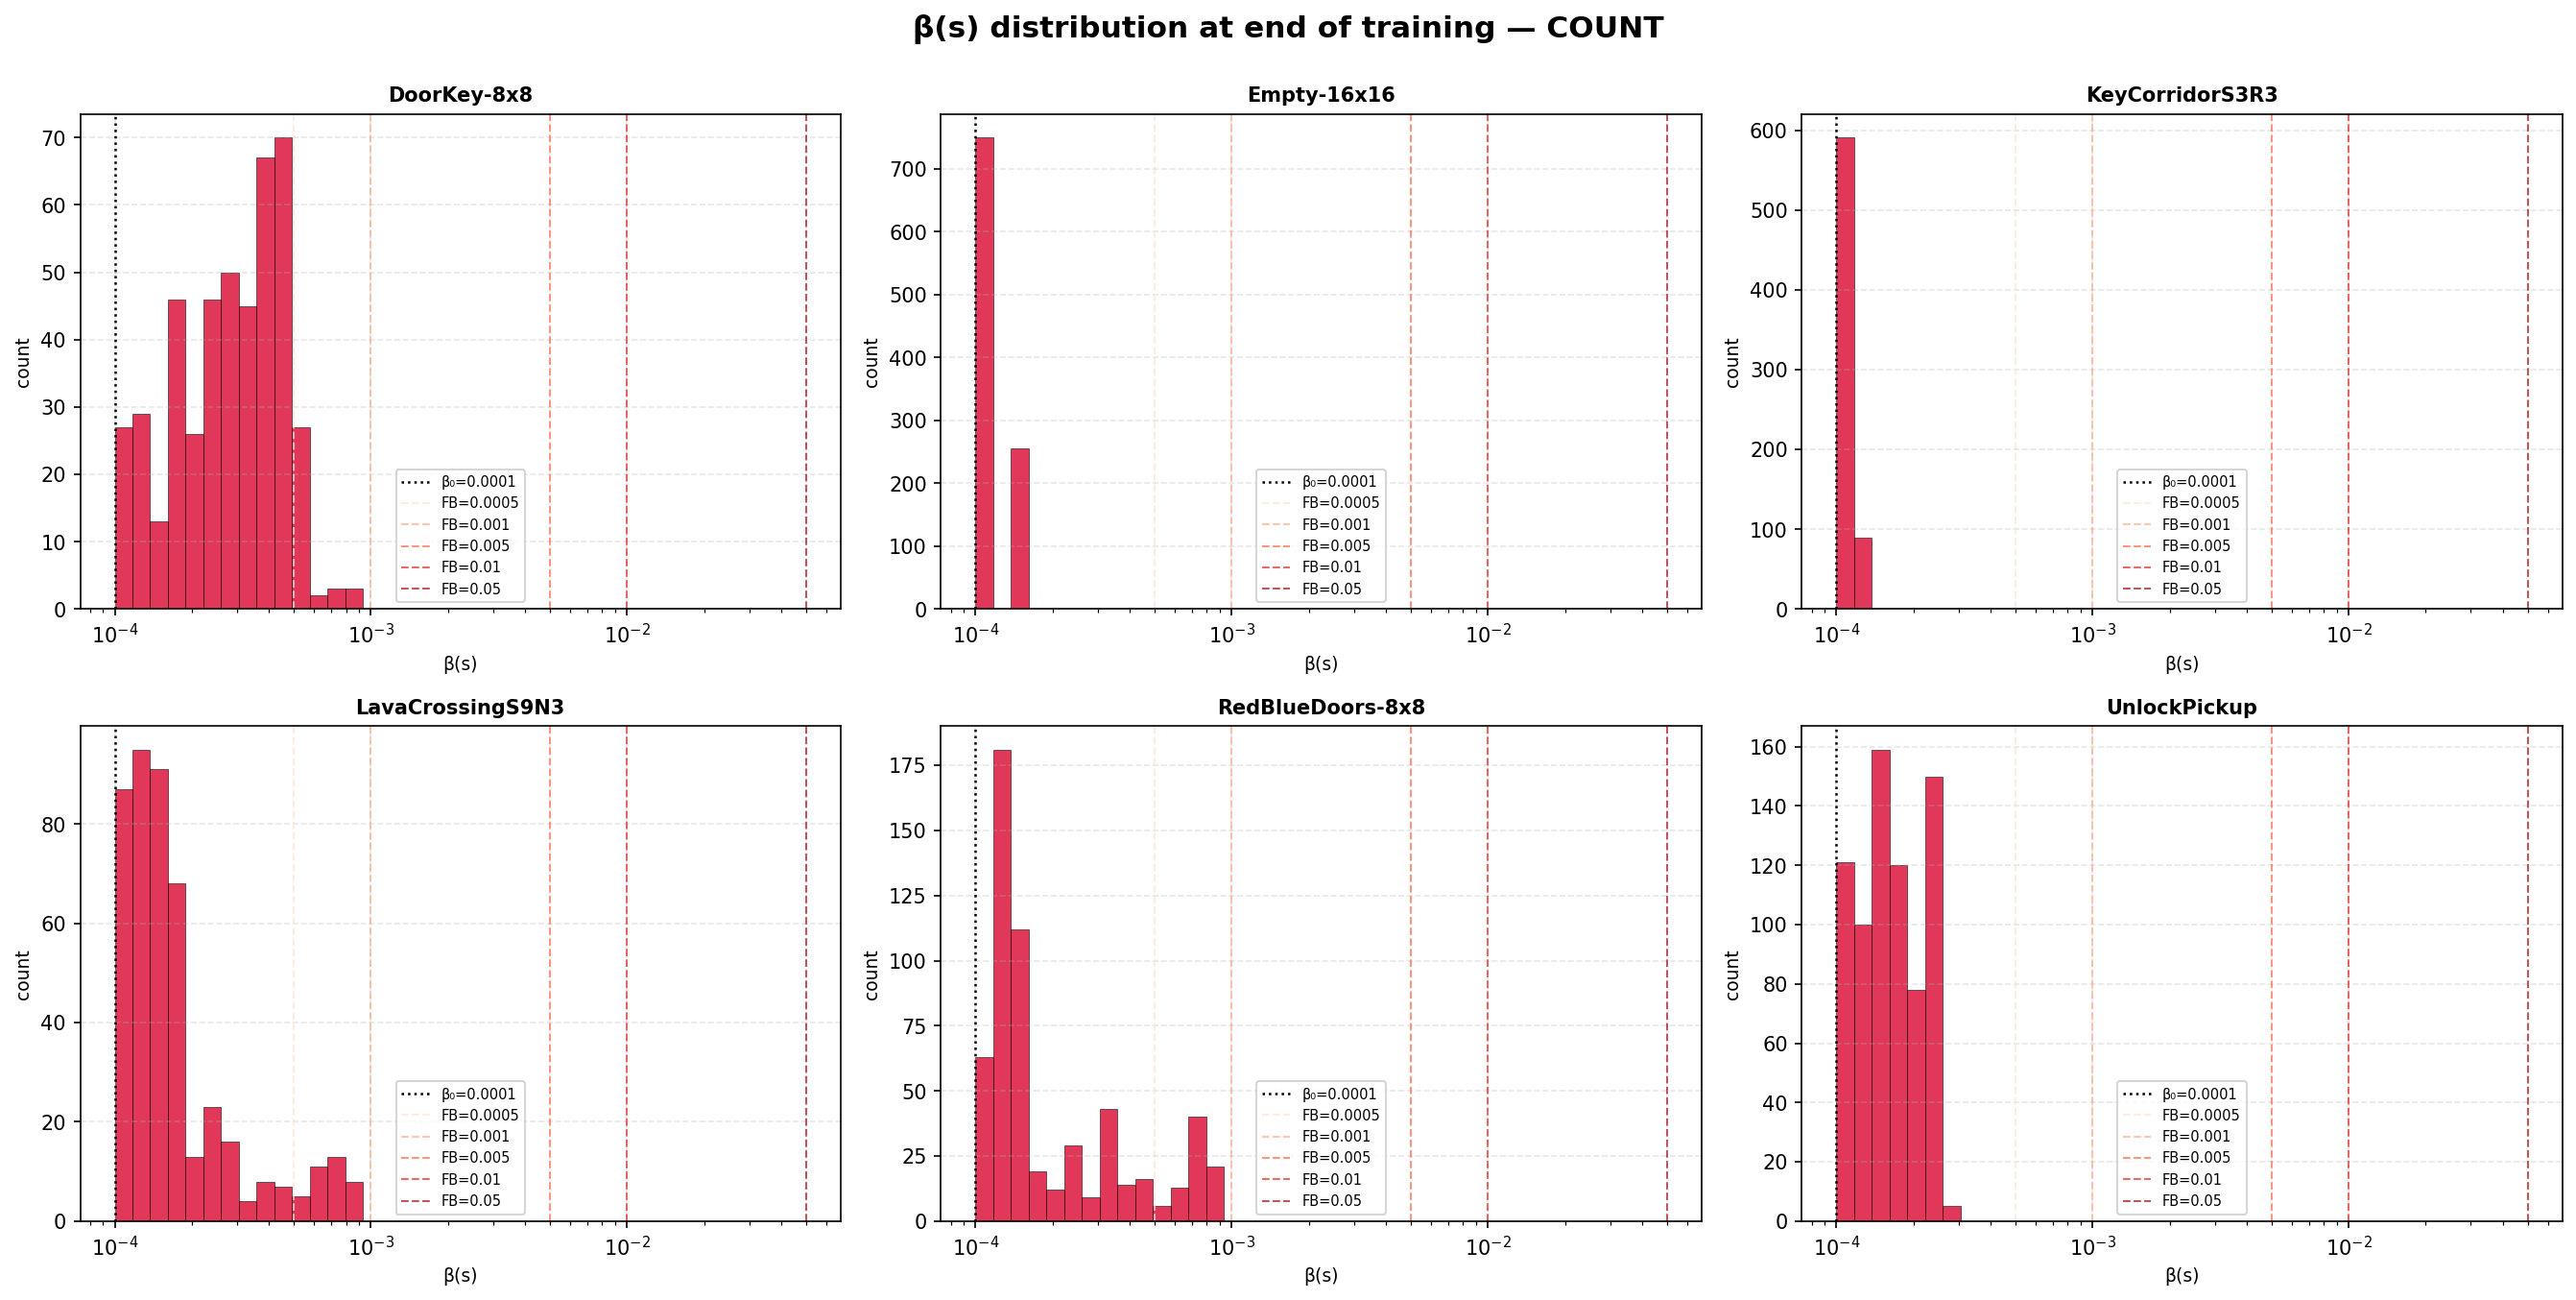
\includegraphics[width=\linewidth]{figures/care_beta_hist_count_beta1e-8_1.png}
\caption[End-of-training $\beta_\psi$ distribution, CARE-COUNT (extended bound).]{End-of-training distribution of $\beta_\psi(s_t)$ for CARE-COUNT under the extended bounds. The reference prior now sits at $\beta_0 = 10^{-4}$, and the histogram x-axis spans $[10^{-8},\,1]$ on a log scale.}
\label{fig:care_beta_hist_count_ext}
\end{figure}

\begin{figure}[H]
\centering
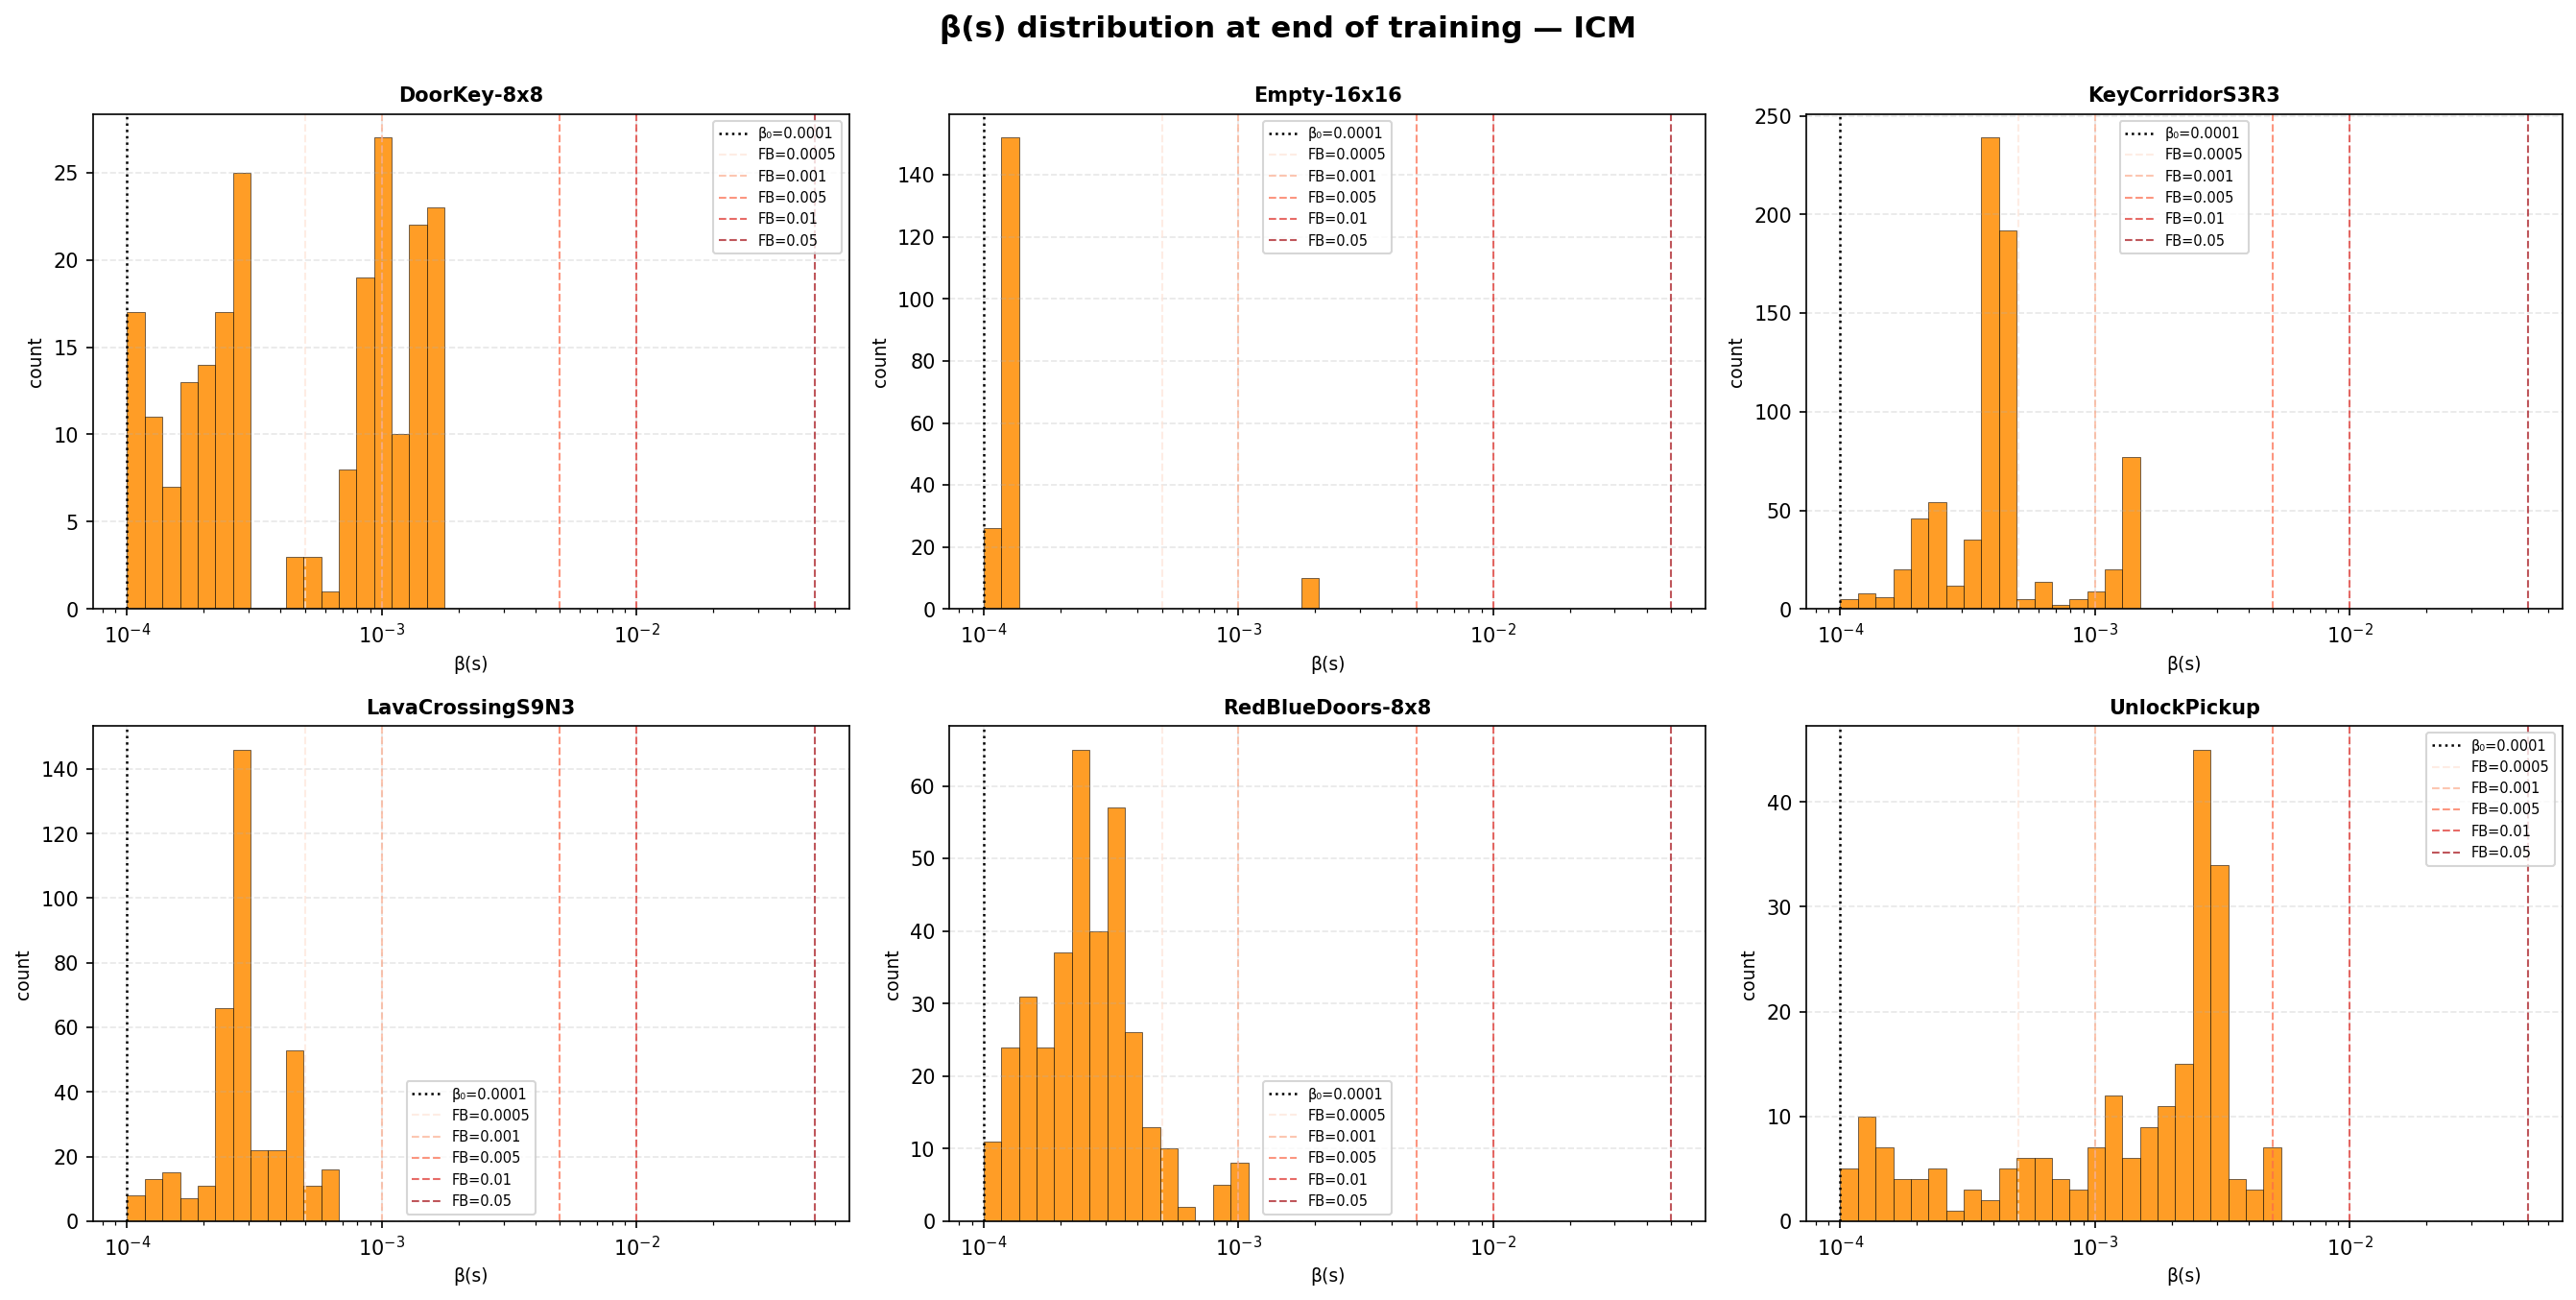
\includegraphics[width=\linewidth]{figures/care_beta_hist_icm_beta1e-8_1.png}
\caption[End-of-training $\beta_\psi$ distribution, CARE-ICM (extended bound).]{End-of-training distribution of $\beta_\psi(s_t)$ for CARE-ICM under the extended bounds. Same conventions as Figure~\ref{fig:care_beta_hist_count_ext}.}
\label{fig:care_beta_hist_icm_ext}
\end{figure}

\begin{figure}[H]
\centering
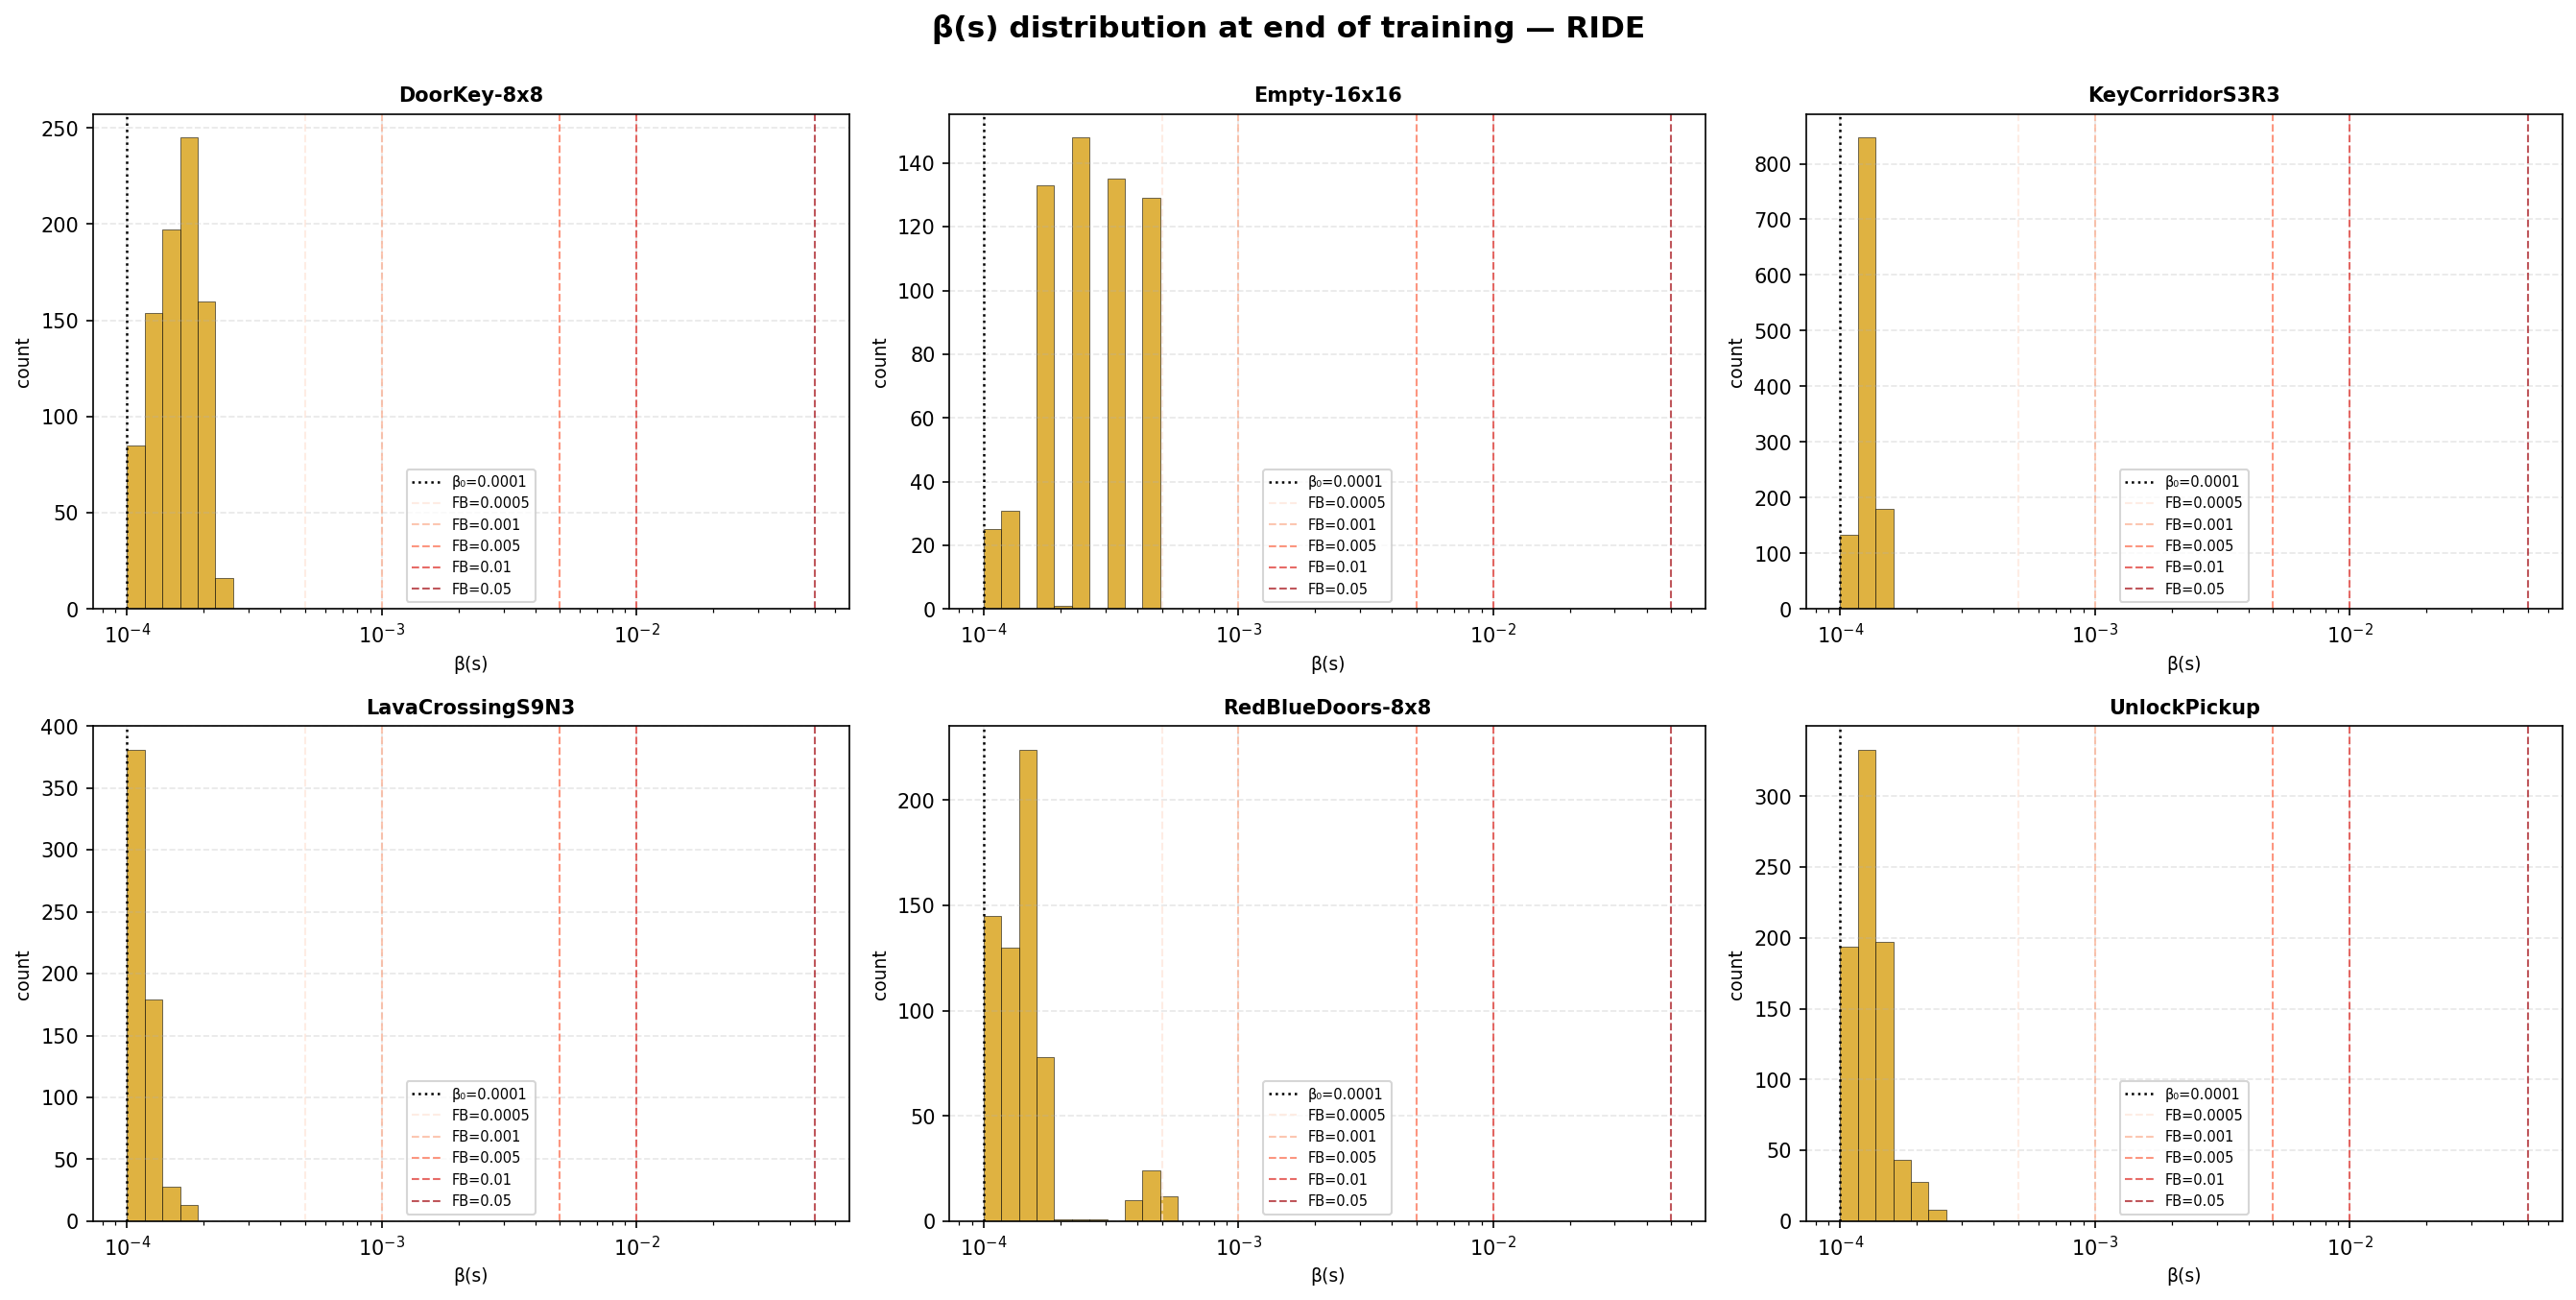
\includegraphics[width=\linewidth]{figures/care_beta_hist_ride_beta1e-8_1.png}
\caption[End-of-training $\beta_\psi$ distribution, CARE-RIDE (extended bound).]{End-of-training distribution of $\beta_\psi(s_t)$ for CARE-RIDE under the extended bounds. Same conventions as Figure~\ref{fig:care_beta_hist_count_ext}.}
\label{fig:care_beta_hist_ride_ext}
\end{figure}

\section{Discussion}
\label{sec:ext_beta_discussion}

Three observations from the figures above are worth recording for comparison with the canonical results in Chapter~\ref{chap:experiment}.

First, the extended bounds shift the cold-start prior from $\beta_0 \approx 2.24 \times 10^{-3}$ down to $\beta_0 = 10^{-4}$, an order-of-magnitude reduction in the initial intrinsic-reward weight. The reward curves in Figures~\ref{fig:all_envs_count_ext}--\ref{fig:all_envs_ride_ext} show that this shift has only a small effect on the easier two environments (DoorKey-8x8 and Empty-16x16), where every condition with non-degenerate $\beta$ converges to near-optimal final reward in either configuration. On the harder four environments (KeyCorridor, LavaCrossing-S9N3, RedBlueDoors-8x8, UnlockPickup) the CARE traces sit somewhat further below the best fixed-$\beta$ envelope than they do in the canonical configuration. The interpretation, consistent with Corollary~\ref{cor:degeneration}(i), is that a much smaller cold-start $\beta_0$ supplies less intrinsic pressure during the long sparse-reward phase before the correlation gradient becomes informative. The canonical $\beta_0 \approx 2.24 \times 10^{-3}$ provides a stronger fallback that the wider bounds give up.

Second, the aggregate view in Figure~\ref{fig:aggregate_summary_ext} and the per-module performance profiles in Figures~\ref{fig:profile_count_ext}--\ref{fig:profile_ride_ext} confirm this asymmetry at the population level. The CARE bars sit at or below the canonical bars in Figure~\ref{fig:aggregate_summary} on the normalized-final-reward axis, and the performance-profile curves of CARE are no higher than in the canonical configuration over most of the $\tau$-range. The wider range therefore does not unlock latent performance that the canonical bounds were suppressing.

Third, the end-of-training histograms in Figures~\ref{fig:care_beta_hist_count_ext}--\ref{fig:care_beta_hist_ride_ext} show where the learned $\beta_\psi(s_t)$ actually settles when given the four extra orders of magnitude on each side. The bulk of the mass stays well inside the canonical interval $[10^{-4},\,5\times 10^{-2}]$ on the environments where CARE converges, with only a thin tail extending into the newly available regions. Combined with the first two observations, this gives an empirical justification for the bounds adopted in Appendix~\ref{app:implementation}: the canonical interval already covers the operating range of the trained $\beta_\psi(s_t)$, and tightening it back from $[10^{-8},\,1]$ to $[10^{-4},\,5\times 10^{-2}]$ improves cold-start behavior without truncating any region of the state space where the learned scaling function would otherwise have placed mass.

Across the three observations, the extended-bounds ablation supports the design choice taken in the main experiments: the canonical $[\beta_\text{min},\,\beta_\text{max}] = [10^{-4},\,5\times 10^{-2}]$ remains the reported configuration for CARE in Chapter~\ref{chap:experiment}.
